\chapter{The Supplied Test Problems}
\label{Sec:The supplied problems}

To verify that Flash-X works as expected and to debug changes in the code, we
have created a suite of standard test problems. Many of these problems have
analytical solutions that can be used to test the accuracy of the code. Most
of the problems that do not have analytical solutions produce
well-defined flow features that have been verified by experiments and are
stringent tests of the code. For the remaining problems, converged solutions,
which can be used to test the accuracy of lower resolution simulations, are
easy to obtain.  The test suite configuration code is included
with the Flash-X source tree (in the \code{Simulation/} directory), so it is easy
to configure and run Flash-X with any of these problems `out of the box.'
Sample runtime parameter files are also included. All the test
problems reside in the \code{Simulations} unit. The unit provides some
general interfaces most of which do not have general
implementations. Each application provides its own implementation for
these interfaces, for example, \code{Simulation\_initBlock}. The
exception is \code{Simulation\_initSpecies}, which provides general
implementations for different classes of problems. 

\section{Hydrodynamics Test Problems}
These problems are primarily designed to test the functioning of the
hydrodynamics solvers within \flashx.

\subsection{Sod Shock-Tube}
\label{Sec:SimulationSod}

The Sod problem (Sod 1978) is a one-dimensional flow
discontinuity problem that provides a good test of a compressible code's
ability to capture shocks and contact discontinuities with a small number of
cells and to produce the correct profile in a rarefaction. It also
tests a code's ability to correctly satisfy the Rankine-Hugoniot shock
jump conditions. When implemented at an angle to a multidimensional grid,
it can be used to detect irregularities in planar discontinuities produced
by grid geometry or operator splitting effects.

We construct the initial conditions for the Sod problem by establishing a
planar interface at some angle to the $x$- and $y$-axes. The fluid is initially
at rest on either side of the interface, and the density and pressure jumps
are chosen so that all three types of nonlinear, hydrodynamic waves
(shock, contact, and rarefaction) develop.
To the ``left'' and ``right'' of the interface we have
\begin{equation}
\begin{array}{lclcclcl}
\rho_{\rm L} &=& 1.0 &   &   & \rho_{\rm R} &=& 0.125\\
p_{\rm L}    &=& 1.0 &   &   & p_{\rm R}    &=& 0.1
\end{array}
\end{equation}
The ratio of specific heats $\gamma$ is chosen to be 1.4 on both sides of
the interface.

In Flash-X, the Sod problem (\code{Sod}) uses the runtime parameters
listed in \tblref{Tab:Sod parameters} in addition to those supplied
by default with the code. For this problem we use the \code{Gamma} equation of
state \childunit and set \rpi{Eos/gamma} to 1.4. The default values listed
in \tblref{Tab:Sod parameters} are appropriate to a shock with
normal parallel to the $x$-axis that initially intersects that axis
at $x=0.5$ (halfway across a box with unit dimensions).
\begin{table}[!ht]

\caption{ Runtime parameters used with the
\code{Sod} test problem.}
\label{Tab:Sod parameters} 
\begin{center}
\begin{tabular}{lllp{3in}}
Variable    & Type      & Default   & Description\\
\hline
\code{sim\_rhoLeft}    & real      & 1     & Initial density to the
                          left of the interface
                          ($\rho_{\rm L}$)\\
\code{sim\_rhoRight}& real     & 0.125     & Initial density to the
                          right ($\rho_{\rm R}$)\\
\code{sim\_pLeft}  & real      & 1     & Initial pressure to the
                          left ($p_{\rm L}$)\\
\code{sim\_pRight} & real      & 0.1       & Initial pressure to the
                          right ($p_{\rm R}$)\\
\code{sim\_uLeft}  & real      & 0     & Initial velocity
                          (perpendicular to interface)
                          to the left ($u_{\rm L}$)\\
\code{sim\_uRight} & real      & 0     & Initial velocity
                          (perpendicular to interface)
                          to the right ($u_{\rm R}$)\\
\code{sim\_xangle}   & real      & 0     & Angle made by interface
                          normal with the $x$-axis
                          (degrees)\\
\code{sim\_yangle}   & real      & 90        & Angle made by interface
                          normal with the $y$-axis
                          (degrees)\\
\code{sim\_posn} & real      & 0.5       & Point of intersection between
                          the interface plane and the
                          $x$-axis\\
\hline
\end{tabular}
\end{center}

\end{table}

\begin{figure}
\begin{center}
{\leavevmode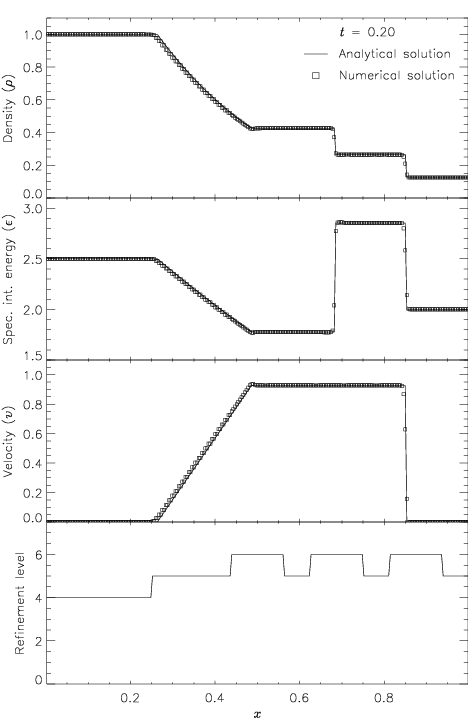
\includegraphics[width=5in]{Sod_single}}
\end{center}
\caption{\label{Fig:Sod single} Comparison of numerical and analytical
solutions to the Sod problem. A 2D grid with six levels of refinement
is used. The shock normal is parallel to the $x$-axis.
}
\end{figure}
\begin{figure}
\begin{center}
{\leavevmode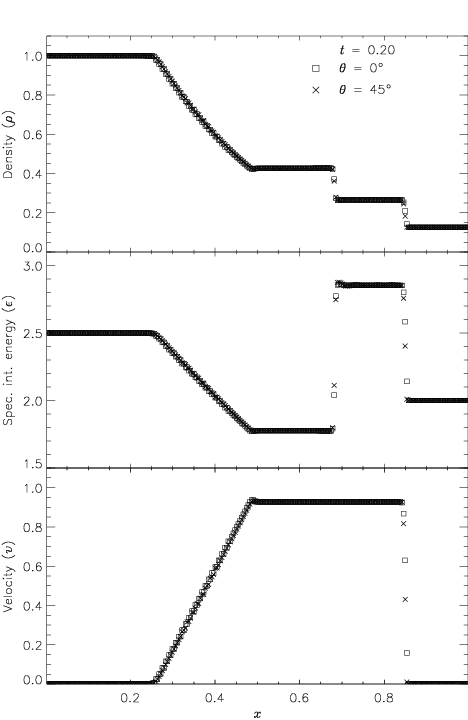
\includegraphics[width=5in]{Sod_compare}}
\end{center}
\caption{\label{Fig:Sod comparison} Comparison of numerical
solutions to the Sod problem for two different angles ($\theta$) of the
shock normal relative to the $x$-axis. A 2D grid with six levels of
refinement is used.
}
\end{figure}

\figref{Fig:Sod single} shows the result of running the Sod problem
with Flash-X on a two-dimensional grid with the analytical solution
shown for comparison. The hydrodynamical algorithm used here is the
directionally split piecewise-parabolic method (PPM) included with
Flash-X. In this run the shock normal is chosen to be parallel to the
$x$-axis. With six levels of refinement, the effective grid size at
the finest level is $256^2$, so the finest cells have width
0.00390625. At $t=0.2$, three different nonlinear waves are present:
a rarefaction between $x = 0.263$ and $x = 0.486$, a contact
discontinuity at $x = 0.685$, and a shock at $x = 0.850$. The two
discontinuities are resolved with approximately two to three cells
each at the highest level of refinement, demonstrating the ability
of PPM to handle sharp flow features well. Near the contact
discontinuity and in the rarefaction, we find small errors of about
$1-2\%$ in the density and specific internal energy, with similar
errors in the velocity inside the rarefaction. Elsewhere, the
numerical solution is close to exact; no oscillations are present.

\figref{Fig:Sod comparison} shows the result of running the Sod
problem on the same two-dimensional grid with different shock
normals: parallel to the $x$-axis ($\theta=0^\circ$) and along the
box diagonal ($\theta=45^\circ$). For the diagonal solution, we have
interpolated values of density, specific internal energy, and
velocity to a set of 256 points spaced exactly as in the $x$-axis
solution. This comparison shows the effects of the second-order
directional splitting used with Flash-X on the resolution of shocks.
At the right side of the rarefaction and at the contact
discontinuity, the diagonal solution undergoes slightly larger
oscillations (on the order of a few percent) than the $x$-axis
solution. Also, the value of each variable inside the discontinuity
regions differs between the two solutions by up to 10\%. However,
the location and thickness of the discontinuities is the same for
the two solutions. In general, shocks at an angle to the grid are
resolved with approximately the same number of cells as shocks
parallel to a coordinate axis.

\figref{Fig:Sod density} presents a colormap plot of the density at
$t=0.2$ in the diagonal solution together with the block structure
of the AMR grid. Note that regions surrounding the discontinuities
are maximally refined, while behind the shock and contact
discontinuity, the grid has de-refined, because the second
derivative of the density has decreased in magnitude. Because
zero-gradient outflow boundaries were used for this test, some
reflections are present at the upper left and lower right corners,
but at $t=0.2$ these have not yet propagated to the center of the
grid.

\begin{figure}[!ht]
\begin{center}
{\leavevmode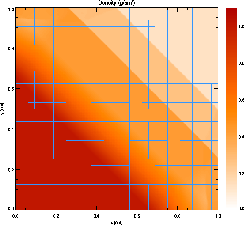
\includegraphics[width=3in]{Sod_2d_density}}
\end{center}
\caption{\label{Fig:Sod density} Density in the diagonal 2D Sod problem
with six levels of refinement at $t=0.2$. The outlines of AMR blocks are
shown (each block contains $8\times8$ cells).
}
\end{figure}

\begin{flashtip}[\code{SodStep} Example]
\flashx also contains under the name \code{SodStep}
a variant of the \code{Sod} problem. This setup is provided as an example for
setting up simulations on domains with steps and obstacles. See
the files in the \code{SodStep} simulation directory
and the \api{Simulation/Simulation_defineDomain} description for 
more information on how to use this feature.
\end{flashtip}

\subsection{Variants of the Sod Problem in Curvilinear Geometries}
\label{Sec:SimulationSodCurvi}
Variants of the \code{Sod} problems can be set up in in various 
geometries in order to test the handling of non-Cartesion geometries.

\begin{itemize}
\item
An axisymmetric variant of the Sod problem can be configured by
setting up the regular \code{Sod} simulation with 
\code{./setup Sod -auto -2d -geometry=cylindrical} and using runtime parameters
that include \code{geometry = "cylindrical"}. 
Use \code{sim_xangle = 0}
to configure an initial shock front that is shaped like a cylinder.
Results as in those discussed in Toro 1999 can be obtained.
\item
A spherically symmetric variant of the Sod problem can be configured by
setting up the regular \code{Sod} simulation with 
\code{./setup Sod -auto -1d -geometry=spherical} and using runtime parameters
that include \code{geometry = "spherical"}.
Again results as in those discussed in Toro 1999 can be obtained.
\item
To test the behavior of Flash-X solutions when the physical symmetry of the
problem does not match the geometry of the simulation,
a separate simulation is provided under the name \code{SodSpherical}.
To use this, configure with \code{./setup SodSpherical -auto -2d -geometry=spherical}
 and using runtime parameters
that include \code{geometry = "spherical"}.
As a 2D setup, \code{SodSpherical} represents physically axisymmetric
initial conditions in spherical coordinates. The physical problem
can be chosen to be the same as in the previous case with cylindrical \code{Sod}.
Again results as in those discussed in Toro 1999 can be obtained.
\item
The \code{SodSpherical} setup can also configured in 1D and will act
like the 1D \code{Sod} setup in that case.
\end{itemize}

%-------------------------------------------------------------------------------

\subsection{Interacting Blast-Wave \code{Blast2}}
\label{Sec:SimulationBlast2}

This \code{Blast2} problem was originally used by Woodward and Colella (1984) to
compare the performance of several different hydrodynamical methods
on problems involving strong shocks and narrow features. It has no analytical
solution (except at very early times), but since it is one-dimensional, it
is easy to produce a converged solution by running the code with a very large
number of cells,
permitting an estimate of the self-convergence rate.
For Flash-X, it also provides a
good test of the adaptive mesh refinement scheme.

The initial conditions consist of two parallel, planar flow discontinuities.
Reflecting boundary conditions are used. The density
is unity and the velocity is zero everywhere.
The pressure is large at the left and right and small in the center
\begin{equation}
\begin{array}{lclcclclcclcl}
p_{\rm L}    &=& 1000, &&    p_{\rm M} &=& 0.01, && p_{\rm R}    &=& 100\ .
\end{array}
\end{equation}
The equation of state is that of a perfect gas with $\gamma=1.4$.

\figref{Fig:WC solution} shows the density and velocity profiles at
several different times in the converged solution, demonstrating the
complexity inherent in this problem. The initial pressure
discontinuities drive shocks into the middle part of the grid;
behind them, rarefactions form and propagate toward the outer
boundaries, where they are reflected back into the grid. By the time
the shocks collide at $t=0.028$, the reflected rarefactions have
caught up to them, weakening them and making their post-shock
structure more complex. Because the right-hand shock is initially
weaker, the rarefaction on that side reflects from the wall later,
so the resulting shock structures going into the collision from the
left and right are quite different. Behind each shock is a contact
discontinuity left over from the initial conditions (at $x\approx
0.50$ and 0.73). The shock collision produces an extremely high and
narrow density peak. The peak density should be slightly less than
30.  However, the peak density shown in \figref{Fig:WC solution} is
only about 18, since the maximum value of the density does not occur
at exactly $t=0.028$. Reflected shocks travel back into the
colliding material, leaving a complex series of contact
discontinuities and rarefactions between them. A new contact
discontinuity has formed at the point of the collision ($x\approx
0.69$). By $t=0.032$, the right-hand reflected shock has met the
original right-hand contact discontinuity, producing a strong
rarefaction, which meets the central contact discontinuity at
$t=0.034$. Between $t=0.034$ and $t=0.038$, the slope of the density
behind the left-hand shock changes as the shock moves into a region
of constant entropy near the left-hand contact discontinuity.
\begin{figure}
\begin{center}
{\leavevmode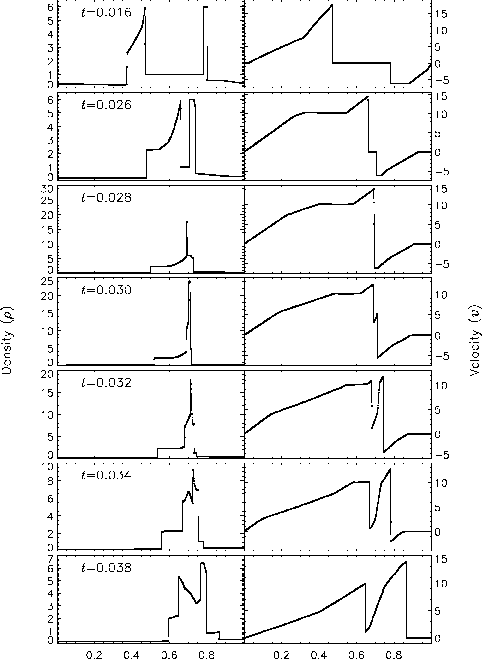
\includegraphics[width=5in]{Blast2_soln}}
\end{center}
\caption{\label{Fig:WC solution} Density and velocity
profiles in the Woodward-Colella
interacting blast-wave problem \code{Blast2} as computed by Flash-X using ten levels of
refinement.
}
\end{figure}

\figref{Fig:WC convergence} shows the self-convergence of density
and pressure when Flash-X is run on this problem. We compare the
density, pressure, and total specific energy at $t=0.038$ obtained
using Flash-X with ten levels of refinement to solutions using several
different maximum refinement levels. This figure plots the L1 error
norm for each variable $u$, defined using
\begin{equation}
\label{Eqn:L1 error norm}
{\cal E}(N_{\rm ref};u) \equiv {1\over N(N_{\rm ref})}
\sum_{i=1}^{N(N_{\rm ref})}\left|{u_i(N_{\rm ref}) -
A
    u_i(10)\over u_i(10)}\right|\ ,
\end{equation}
against the effective number of cells
($N(N_{\rm ref})$).
In computing this norm, both the `converged' solution $u(10)$ and
the test solution $u(N_{\rm ref})$ are interpolated onto a uniform
mesh having $N(N_{\rm ref})$ cells.
Values of
$N_{\rm ref}$ between 2 (corresponding to cell size $\Delta x=1/16$)
and 9 ($\Delta x=1/2048$) are shown.

Although PPM is formally a second-order method, the convergence rate is
only linear. This is not surprising, since the order of accuracy of a method
applies only to smooth flow and not to flows containing discontinuities.
In fact, all shock capturing schemes are only first-order accurate in the
vicinity of discontinuities.  Indeed, in their comparison of the performance
of seven nominally second-order hydrodynamic
methods on this problem, Woodward and Colella found that only PPM achieved
even linear convergence; the other methods were worse. The error norm
is very sensitive to the correct position and shape of the strong, narrow
shocks generated in this problem.

The additional runtime parameters supplied with the \code{2blast}
problem are listed in \tblref{Tab:WC parameters}. This problem is
configured to use the perfect-gas equation of state (\code{gamma})
with \code{gamma} set to 1.4 and is run in a two-dimensional unit
box. Boundary conditions in the $y$-direction (transverse to the
shock normals) are taken to be periodic.

\vfill
\eject

\begin{center}
\begin{longtable}{lllp{3in}}

\caption{ Runtime parameters used with the
\code{2blast} test problem.} \\
\label{Tab:WC parameters}
Variable    & Type      & Default   & Description\\
\hline
\code{rho\_left}    & real      & 1     & Initial density to the
                          left of the left interface
                          ($\rho_{\rm L}$)\\
\code{rho\_mid} & real      & 1     & Initial density between
                          the two interfaces
                          ($\rho_{\rm M}$)\\
\code{rho\_right}& real     & 1     & Initial density to the
                          right of the right
                          interface
                          ($\rho_{\rm R}$)\\
\code{p\_left}  & real      & 1000      & Initial pressure to the
                          left ($p_{\rm L}$)\\
\code{p\_mid}   & real      & 0.01      & Initial pressure in the
                          middle ($p_{\rm M}$)\\
\code{p\_right} & real      & 100       & Initial pressure to the
                          right ($p_{\rm R}$)\\
\code{u\_left}  & real      & 0     & Initial velocity
                          (perpendicular to interface)
                          to the left ($u_{\rm L}$)\\
\code{u\_mid}   & real      & 0     & Initial velocity
                          (perpendicular to interface)
                          in the middle ($u_{\rm M}$)\\
\code{u\_right} & real      & 0     & Initial velocity
                          (perpendicular to interface)
                          to the right ($u_{\rm R}$)\\
\code{xangle}   & real      & 0     & Angle made by interface
                          normal with the $x$-axis
                          (degrees)\\
\code{yangle}   & real      & 90        & Angle made by interface
                          normal with the $y$-axis
                          (degrees)\\
\code{posnL}    & real      & 0.1       & Point of intersection between
                          the left interface plane
                          and the
                          $x$-axis\\
\code{posnR}    & real      & 0.9       & Point of intersection between
                          the right interface plane
                          and the
                          $x$-axis\\
\hline

\end{longtable}
\end{center}

\begin{figure}
\begin{center}
{\leavevmode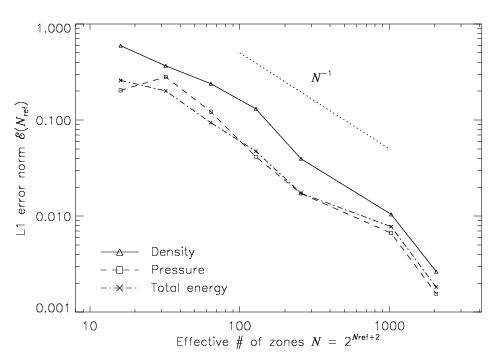
\includegraphics[width=5in]{Blast2_conv}}
\end{center}
\caption{\label{Fig:WC convergence} Self-convergence of the density,
pressure, and total specific energy in the \code{Blast2} test problem.
}
\end{figure}

%-------------------------------------------------------------------------------

\subsection{Sedov Explosion}
\label{Sec:SimulationSedov}

The Sedov explosion problem (Sedov 1959) is another purely hydrodynamical
test in which we check the code's ability to deal with strong shocks
and non-planar symmetry. The problem involves the self-similar evolution
of a cylindrical or
spherical blast wave from a delta-function initial pressure perturbation
in an otherwise homogeneous medium. 
We provide two different ways to generate the initial conditions:
\begin{enumerate}
\item
We deposit a quantity of energy $E=1$ into a
small region of radius $\delta r$ at the center of the grid.
The pressure inside this volume $p_0'$ is given by
\begin{equation}
p_0' = {3(\gamma-1)E\over(\nu+1)\pi\,\delta r^\nu}\ ,
\end{equation}
\noindent where $\nu=2$ for cylindrical geometry and $\nu=3$ for spherical
geometry. 
\item
We initialize from a precomputed pseudo-analytical solution by reading
in a 1D profile.
\end{enumerate}

We set the ratio of specific heats $\gamma=1.4$.
In running this problem we choose $\delta r$ to be 3.5
times as large as the finest adaptive mesh resolution in order to minimize
effects due to the Cartesian geometry of our grid.
The density
is set equal to $\rho_0=1$ everywhere, and the
pressure is set to a small value $p_0=10^{-5}$ everywhere but in the center
of the grid.
The fluid is initially at rest.
In the self-similar blast wave that develops for $t>0$, the
density, pressure, and radial velocity are all functions of
$\xi \equiv r/R(t)$, where
\begin{equation}
R(t) = C_\nu(\gamma) \left({Et^2\over \rho_0}\right)^{1/(\nu+2)}\ .
\end{equation}
\noindent Here $C_\nu$ is a
dimensionless constant depending only on $\nu$ and $\gamma$; for
$\gamma=1.4$, $C_2 \approx C_3 \approx 1$ to within a few percent.
Just behind the shock front at $\xi = 1$ the analytical solution is
\begin{eqnarray}
\nonumber
\rho = & \rho_1\,\, \equiv & {\gamma+1\over\gamma-1}\rho_0 \\
p    = & p_1\,\,    \equiv & {2\over\gamma+1}\rho_0 u^2 \\
\nonumber
v    = & v_1\,\,    \equiv & {2\over\gamma+1}u\ ,
\end{eqnarray}
\noindent where $u \equiv dR/dt$ is the speed of the shock wave. Near the
center of the grid,
\begin{eqnarray}
\nonumber
\rho(\xi)/\rho_1 & \propto & \xi^{\nu/(\gamma-1)} \\
p(\xi)/p_1       & =       & {\rm constant}\ \\
\nonumber
v(\xi)/v_1       & \propto & \xi \ .
\end{eqnarray}

\begin{figure}
\begin{center}
{\leavevmode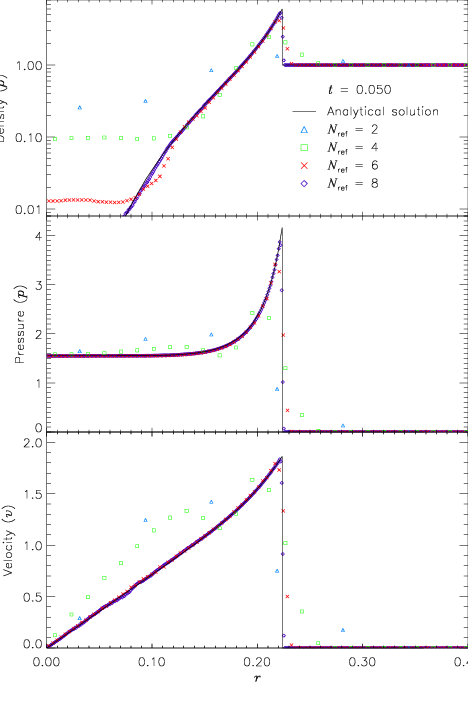
\includegraphics[width=5in]{Sedov_2d_compare}}
\end{center}
\caption{\label{Fig:Sedov compare} Comparison of numerical and analytical
solutions to the Sedov problem in two dimensions. Numerical solution values
are averages in radial bins at the finest AMR grid resolution $N_{\rm ref}$ in each run.
}
\end{figure}
\figref{Fig:Sedov compare} shows density, pressure, and velocity
profiles in the two-dimensional, cylindrical Sedov problem at
$t=0.05$. Solutions obtained with Flash-X on grids with 2, 4, 6, and 8
levels of refinement are shown in comparison with the analytical
solution. In this figure we have computed average radial profiles in
the following way. We interpolated solution values from the
adaptively gridded mesh used by Flash-X onto a uniform mesh having the
same resolution as the finest AMR blocks in each run. Then, using
radial bins with the same width as the cells in the uniform mesh, we
binned the interpolated solution values, computing the average value
in each bin. At low resolutions, errors show up as density and
velocity overestimates behind the shock, underestimates of each
variable within the shock, and a very broad shock structure.
However, the central pressure is accurately determined, even for two
levels of refinement. Because the density goes to a finite value
rather than to its correct limit of zero, this corresponds to a
finite truncation of the temperature (which should go to infinity as
$r\rightarrow 0$).  This error results from depositing the initial
energy into a finite-width region rather than starting from a delta
function. As the resolution improves and the value of $\delta r$
decreases, the artificial finite density limit also decreases; by
$N_{\rm ref}=6$ it is less than 0.2\% of the peak density. Except
for the $N_{\rm ref}=2$ case, which does not show a well-defined
peak in any variable, the shock itself is always captured with about
two cells. The region behind the shock containing 90\% of the
swept-up material is represented by four cells in the $N_{\rm
ref}=4$ case, 17 cells in the $N_{\rm ref}=6$ case, and 69 cells for
$N_{\rm ref}=8$. However, because the solution is self-similar, for
any given maximum refinement level, the structure will be four cells
wide at a sufficiently early time. The behavior when the shock is
under-resolved is to underestimate the peak value of each variable,
particularly the density and pressure.

\figref{Fig:Sedov refinement} shows the pressure field in the
8-level calculation at $t=0.05$ together with the block refinement
pattern. Note that a relatively small fraction of the grid is
maximally refined in this problem. Although the pressure gradient at
the center of the grid is small, this region is refined because of
the large temperature gradient there. This illustrates the ability
of \Paramesh to refine grids using several different variables at
once.
\begin{figure}[!ht]
\begin{center}
{\leavevmode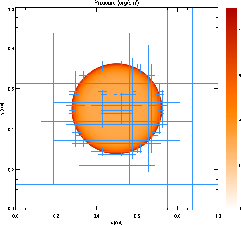
\includegraphics[width=3in]{Sedov_pressure}}
\end{center}
\caption{\label{Fig:Sedov refinement} Pressure field in the
2D Sedov explosion problem with 8 levels of refinement at $t=0.05$.
The outlines of the AMR blocks are overlaid on the pressure colormap.
}
\end{figure}


%In \figref{Fig:Sedov convergence}
%we plot the pressure error norm ([\eqref{Eqn:L1 error norm}]) for
%these results as a function of the effective number of cells.
%Note that here we are measuring the accuracy of the code, rather than
%the self-convergence rate, because we measure errors against the
%analytical solution. ...
%
%\begin{figure}
%\begin{center}
%%{\leavevmode\includegraphics[width=5in]{Sedov_2d_conv}}
%\end{center}
%\caption{\label{Fig:Sedov convergence} Convergence of the
%pressure in the two-dimensional \code{sedov} test problem.
%}
%\end{figure}

We have also run Flash-X on the spherically symmetric Sedov problem in
order to verify the code's performance in three dimensions. The
results at $t=0.05$ using five levels of grid refinement are shown
in \figref{Fig:Sedov 3D single}. In this figure we have plotted the
average values as well as the root-mean-square (RMS) deviations from
the averages. As in the two-dimensional runs, the shock is spread
over about two cells at the finest AMR resolution in this run. The
width of the pressure peak in the analytical solution is about 1~1/2
cells at this time, so the maximum pressure is not captured in the
numerical solution. Behind the shock the numerical solution average
tracks the analytical solution quite well, although the Cartesian
grid geometry produces RMS deviations of up to 40\% in the density
and velocity in the de-refined region well behind the shock. This
behavior is similar to that exhibited in the two-dimensional problem
at comparable resolution.
\begin{figure}
\begin{center}
{\leavevmode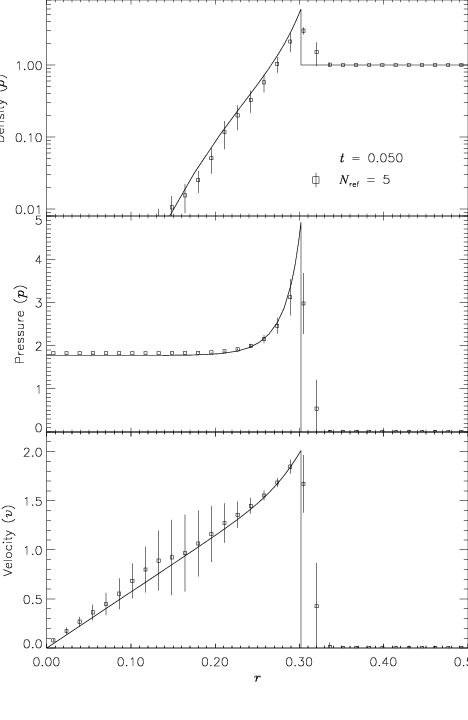
\includegraphics[width=5in]{Sedov_3d_single}}
\end{center}
\caption{\label{Fig:Sedov 3D single} Comparison of numerical and analytical
solutions versus radius $r$ to the spherically symmetric Sedov problem. A 3D grid with
five levels of refinement is used.
}
\end{figure}

The additional runtime parameters supplied with the \code{Sedov}
problem are listed in \tblref{Tab:Sedov parameters}. This problem is
configured to use the perfect-gas equation of state (\code{Gamma})
with \rpi{Eos/gamma} set to 1.4.  It is simulated in a unit-sized box.

\begin{table}

\caption{ Runtime parameters used with the
\code{Sedov} test problem.}
\label{Tab:Sedov parameters} 
\begin{center}
\begin{tabular}{lllp{3in}}
Variable    & Type      & Default   & Description\\
\hline
\code{sim\_pAmbient}& real     & $10^{-5}$ & Initial ambient pressure
                          ($p_0$)\\
\code{sim\_rhoAmbient}
        & real      & 1     & Initial ambient density
                          ($\rho_0$)\\
\code{sim\_expEnergy}
        & real      & 1     & Explosion energy ($E$)\\
\code{sim\_rInit}  & real      & 0.05      & Radius of initial pressure
                          perturbation ($\delta r$)\\
\code{sim\_xctr} & real      & 0.5       & $x$-coordinate of explosion
                          center\\
\code{sim\_yctr} & real      & 0.5       & $y$-coordinate of explosion
                          center\\
\code{sim\_zctr} & real      & 0.5       & $z$-coordinate of explosion
                          center\\
\code{sim\_nSubZones} & integer & 7 & Number of sub-cells in cells for applying the 1D profile \\
\hline
\end{tabular}
\end{center}

\end{table}

\subsubsection{Sedov Self-Gravity}
\label{Sec:SimulationSedovSelfGravity}
Another variant of the Sedov problem is included in the release which
runs with spherical coordinates in one dimension. The \code{Sedov
Self-Gravity} problem also allows the effects of gravitational
acceleration where the gravitational potential is calculated using the
multipole solver. \figref{Fig:Sedov_sg1} and \ref{Fig:Sedov_sg2}
show the snapshots of the density profile and the gravitational
potential at two different times during the evolution. The first
snapshot is at $t=0.5$ sec, when evolution is halfway through, while the
second snapshot is at the end of the evolution, where $t=1.0$ sec.
\begin{figure}
{\leavevmode\includegraphics[width=3.2in]{sedov_sg_dens1}}
{\leavevmode\includegraphics[width=3.2in]{sedov_sg_gpot1}}
\caption{\label{Fig:Sedov_sg1} Snapshots of Sedov Self-gravity
density profile and gravitational potential at time t=0.5 sec.}
\end{figure}

\begin{figure}
{\leavevmode\includegraphics[width=3.2in]{sedov_sg_dens2}}
{\leavevmode\includegraphics[width=3.2in]{sedov_sg_gpot2}}
\caption{\label{Fig:Sedov_sg2} Snapshots of Sedov Self-gravity
density profile and gravitational potential at time t=1.0 sec.}

\end{figure}

\newpage
%% \subsection{The Advection Problem \code{Advect}}

%% In the \code{Advect} problem we create a planar density pulse in a region of
%% uniform pressure $p_0$ and velocity ${\bf u}_0$, with the velocity normal to
%% the pulse plane. The density pulse is defined via
%% \begin{equation}
%% \rho(s) = \rho_1\phi(s/w) + \rho_0\left[1-\phi(s/w)\right]\ ,
%% \end{equation}
%% where $s$ is the distance of a point from the pulse midplane, $w$ is
%% the characteristic width of the pulse, and the pulse shape function
%% $\phi$ is
%% \begin{equation}
%% \phi_{\rm SP}(\xi) = \left\{ \begin{array}{l@{\quad}l}
%%                 1   & |\xi|<1 \\
%%                 0   & |\xi|>1
%%                  \end{array} \right.\ ,
%% \end{equation}
%% for a square pulse and
%% \begin{equation}
%% \phi_{\rm GP}(\xi) = e^{-\xi^2}\ ,
%% \end{equation}
%% for a Gaussian pulse.
%% For these initial conditions, the Euler equations reduce to a single
%% advection equation with propagation speed $u_0$; hence the density pulse should
%% move across the computational volume at this speed without changing
%% shape. Advection problems similar to this were first proposed by
%% Boris and Book (1973) and Forester (1977).

%% Like the Sod problem, the advection problem tests the ability of the code
%% to handle planar geometry and the code's treatment of contact
%% discontinuities.  In some ways, contact discontinuities are the most
%% difficult type of hydrodynamic wave for a shock capturing code to get
%% right.  Shocks contain a self-steepening mechanism, so diffusive
%% errors that tend to spread the shock structure do so only up to a certain
%% limit.  However, contact discontinuities are not self-steepening, so any
%% artificial diffusion in the numerical method will continue to spread the
%% discontinuity throughout the calculation.  In addition,
%% any numerical noise generated at a contact discontinuity tends to move with
%% the interface, accumulating there as the calculation advances.
%% The advection problems presented here compare the code's treatment of both
%% leading and trailing contact discontinuities (for the square pulse)
%% and the treatment of narrow flow features (for both the square and for the
%% Gaussian pulse shapes). Many hydrodynamical methods have a tendency to clip
%% narrow features or to distort pulse shapes by introducing artificial
%% dispersion and dissipation (Zalesak 1987).


%% \begin{table}

%% \caption{ \label{Tab:Advection parameters} Runtime parameters used with the
%% \code{Advect} test problem.}

%% \begin{center}
%% \begin{tabular}{lllp{3in}}
%% Variable    & Type      & Default   & Description\\
%% \hline
%% \code{sim\_rhoIn}    & real      & 1     & Characteristic density
%%                           inside the advected pulse
%%                           ($\rho_1$)\\
%% \code{sim\_rhoOut}   & real      & $10^{-5}$ & Ambient density
%%                           ($\rho_0$)\\
%% \code{sim\_pressure} & real      & 1     & Ambient pressure ($p_0$)\\
%% \code{sim\_velocity} & real      & 10        & Ambient velocity ($u_0$)\\
%% \code{sim\_width}    & real      & 0.1       & Characteristic
%%                           width of advected pulse
%%                           ($w$)\\
%% \code{sim\_pulseFunctn}
%%         & integer   & 1     & Pulse shape function to
%%                           use: 1=square wave,
%%                           2=Gaussian\\
%% \code{sim\_xAngle}   & real      & 0     & Angle made by pulse plane
%%                           with $x$-axis (degrees)\\
%% \code{sim\_yAngle}   & real      & 90        & Angle made by pulse plane
%%                           with $y$-axis (degrees)\\
%% \code{sim\_posn} & real      & 0.25      & Point of intersection between
%%                           pulse midplane and $x$-axis
%%                           \\
%% \hline
%% \end{tabular}
%% \end{center}

%% \end{table}

%% The additional runtime parameters supplied with the \code{Advect}
%% problem are listed in \tblref{Tab:Advection parameters}. This
%% problem is configured to use the perfect-gas equation of state
%% (\code{Gamma}) with \rpi{Eos/gamma} set to 1.4 and is run in a unit
%% box. The value of $\gamma$ does not affect the analytical solution,
%% but it does affect the simulation timestep.

%% To demonstrate the performance of Flash-X on the advection problem, we have
%% performed tests of both the square and Gaussian pulse profiles with the
%% pulse normal parallel to the $x$-axis ($\theta=0^\circ$) and at an angle
%% to the $x$-axis ($\theta=45^\circ$) in two dimensions. The square pulse
%% used $\rho_1=1$, $\rho_0=10^{-3}$, $p_0=10^{-6}$, $u_0=1$, and $w=0.1$.
%% With six levels of refinement in the domain $[0,1]\times[0,1]$, this value
%% of $w$ corresponds to having about 52 cells across the pulse width.
%% The Gaussian pulse tests used the same values of $\rho_1$, $\rho_0$, $p_0$,
%% and $u_0$, but with $w=0.015625$. This value of $w$ corresponds to about
%% 8 cells across the pulse width at six levels of refinement. For each test,
%% we performed runs at two, four, and six levels of refinement to examine the
%% quality of the numerical solution as the resolution of the advected pulse
%% improves. The runs with $\theta=0^\circ$ used zero-gradient (outflow)
%% boundary conditions, while the runs performed at an angle to the $x$-axis
%% used periodic boundaries.

%% \figref{Fig:advection} shows the advected density profiles at
%% $t=0.4$ compared to the analytical solution. The upper two frames of
%% this figure depict the square pulse with $\theta=0^\circ$ and
%% $\theta=45^\circ$, while the lower two frames depict the Gaussian
%% pulse results. In each case the analytical density pulse has been
%% advected a distance $u_0t=0.4$. In the figure the axis parallel to
%% the pulse normal has been translated by this amount.
%% \begin{figure}
%% \begin{center}
%% {\leavevmode\includegraphics[width=5in]{Advection}}
%% \end{center}
%% \caption{\label{Fig:advection} Density pulse in the advection tests for
%% 2D grids at $t=0.4$. Symbols represent numerical results using grids with
%% different levels of refinement 
%% $N_{\rm ref}$ 
%% \rpi{Grid/lrefine_max}
%% (2, 4, and 6).
%% }
%% \end{figure}

%% The advection results show the expected improvement with increasing
%% AMR refinement level $N_{\rm ref}$. Inaccuracies appear as diffusive
%% spreading, rounding of sharp corners, and clipping.
%% Both in the square pulse test and in the Gaussian pulse test, diffusive
%% spreading is limited to about one cell on either side of the pulse.
%% For $N_{\rm ref}=2$,
%% the rounding of the square pulse and the clipping of the Gaussian pulse are
%% quite severe; in the latter case, the pulse itself spans about two cells,
%% which is the approximate smoothing length in PPM for a single discontinuity.
%% For $N_{\rm ref}=4$, the treatment of the square pulse is significantly better,
%% but the amplitude of the Gaussian is still reduced by about 50\%.
%% In this case the square pulse discontinuities are still being resolved with
%% 2--3 cells, but the cells are now a factor of 25 smaller than the pulse width.
%% With six levels of refinement, the same behavior is observed for the square
%% pulse, while the amplitude of the Gaussian pulse is now 93\% of its initial
%% value. The absence of dispersive effects (\ie,\ oscillations)
%% despite the high
%% order of the PPM interpolants is due to the enforcement of monotonicity
%% in the PPM algorithm.

%% The diagonal runs are consistent with the runs which were parallel to
%% the $x$-axis, with the possibility of a slight amount of extra spreading
%% behind the pulse. However, note that we have determined
%% density values for the diagonal runs by interpolation
%% along the grid diagonal. The interpolation points are not centered on the
%% pulses, so the density does not always take on its maximum value
%% (particularly in the lowest-resolution case).

%% These results are consistent with earlier studies of linear advection with
%% PPM (e.g., Zalesak 1987). They
%% suggest that, in order to preserve narrow flow features in Flash-X,
%% the maximum AMR refinement level should be chosen so that cells
%% are at least a factor 5--10 smaller than the narrowest features of
%% interest. In cases in which the features are generated by shocks (rather
%% than moving with the fluid), the resolution requirement is not as severe,
%% since errors generated in the preshock region are driven into the shock rather
%% than accumulating as it propagates.


%% \vfill
%% \eject
%% \newpage
\subsection{Isentropic Vortex}
\label{Sec:SimulationIsentropicVortex}

The two-dimensional isentropic vortex problem is often used as a
benchmark for comparing numerical methods for fluid dynamics. The
flow-field is smooth (there are no shocks or contact discontinuities)
and contains no steep gradients, and the exact solution is known. It
was studied by Yee, Vinokur, and Djomehri (2000) and by Shu (1998). In
this subsection the problem is described, the Flash-X control parameters
are explained, and some results demonstrating how the problem can be
used are presented.

The simulation domain is a square, and the center of the vortex is
located at $(x_{ctr}, y_{ctr})$. The flow-field is defined in
coordinates centered on the vortex center $(x' = x - x_{ctr}, y' = y
- y_{ctr})$ with $r^2 = {x'}^2 + {y'}^2$. The domain is periodic, but
it is assumed that off-domain vortexes do not interact with the
primary; practically, this assumption can be
satisfied by ensuring that the simulation domain is large enough for a
particular vortex strength. We find that a domain size of $10 \times
10$ (specified through the \code{Grid} runtime parameters \rpi{Grid/xmin},
\rpi{Grid/xmax}, \rpi{Grid/ymin}, and \rpi{Grid/ymax}) is sufficiently large for a
vortex strength (defined below) of~5.0. In the initialization below,
$x'$ and $y'$ are the coordinates with respect to the nearest vortex
in the periodic sense.

The ambient conditions are given by $\rho_\infty$, $u_\infty$,
$v_\infty$, and $p_\infty$, and the non-dimensional ambient temperature
is $T^*_\infty = 1.0$. Using the equation of state, the (dimensional)
$T_\infty$ is computed from $p_\infty$ and
$\rho_\infty$. Perturbations are added to the velocity and
nondimensionalized temperature, $u = u_\infty + \delta u$, $v =
v_\infty + \delta v$, and $T^* = T^*_\infty + \delta T^*$ according to
\begin{eqnarray}
\label{Eqn:isentropic_three}
\delta u &=&
-y' {\frac {\beta} {2 \pi}} \exp \left( {\frac {1-r^2} {2}} \right) \\
\delta v &=&
 x' {\frac {\beta} {2 \pi}} \exp \left( {\frac {1-r^2} {2}} \right) \\
\delta T^* &=&
- { \frac {(\gamma - 1 ) \beta}  {8 \gamma \pi^2}} \exp \left( {1-r^2}
\right)~,
\end{eqnarray}
where $\gamma=1.4$ is the ratio of specific heats and $\beta=5.0$ is a
measure of the vortex strength. The temperature and density are then given by
\begin{eqnarray}
T &=& {\frac{T_\infty}{T^*_\infty} } T^* \\
\rho &=& \rho_\infty
  \left( {\frac{T}{T_\infty} } \right)^{\frac{1}{\gamma-1} }~.
\end{eqnarray}
At any location in space, the conserved variables (density, $x$- and
$y$-momentum, and total energy) can be computed from the above
quantities.  The flow-field is initialized by computing cell averages
of the conserved variables; in each cell, the average is
approximated by averaging over $\code{nx\_subint} \times
\code{ny\_subint}$ subintervals. The runtime parameters for the
isentropic vortex problem are listed in \tblref{Tab:Isentropic
Vortex parameters}.

\begin{center}
\begin{longtable}{lllp{3.8in}}

\caption{ Parameters
for the \code{IsentropicVortex} problem.} \\
\label{Tab:Isentropic Vortex parameters} 
Variable        & Type          & Default       & Description\\
\hline
\code{p\_ambient}& real          & 1.0           & Initial ambient pressure
                                                  ($p_{\infty}$)\\
\code{rho\_ambient}
                & real          & 1.0           & Initial ambient density
                                                  ($\rho_{\infty}$)\\
\code{u\_ambient}& real          & 1.0           & Initial ambient $x$-velocity
                                                  ($u_{\infty}$)\\
\code{v\_ambient}& real          & 1.0           & Initial ambient $y$-velocity
                                                  ($v_{\infty}$)\\
\code{vortex\_strength}
                & real          & 5.0           & Non-dimensional vortex
                                                  strength \\
\code{xctr}      & real          & 0.0           & $x$-coordinate of vortex
                                                  center\\
\code{yctr}      & real          & 0.0           & $y$-coordinate of vortex
                                                  center\\
\code{nx\_subint}& integer       & 10            & number of subintervals in
                                                  $x$-direction\\
\code{ny\_subint}& integer       & 10            & number of subintervals in
                                                  $y$-direction\\
\hline
\end{longtable}
\end{center}

\figref{Fig:iv1} shows the exact density distribution represented on
a $40 \times 40$ uniform grid with $-5.0 \leq x, y \leq 5.0$. The
borders of each grid block ($8 \times 8$ cells) are superimposed. In
addition to the shaded representation, contour lines are shown for
$\rho = 0.95$, 0.85, 0.75, and 0.65. The density distribution is
radially symmetric, and the minimum density is $\rho_{min} =
0.510287$. Because the exact solution of the isentropic vortex
problem is the initial solution shifted by $(u_\infty t, v_\infty
t)$, numerical phase (dispersion) and amplitude (dissipation) errors
are easy to identify. Dispersive errors distort the shape of the
vortex, breaking its symmetry.  Dissipative errors smooth the
solution and flatten extrema; for the vortex, the minimum in density
at the vortex core will increase.
\begin{figure}[!ht]
\begin{center}
{\leavevmode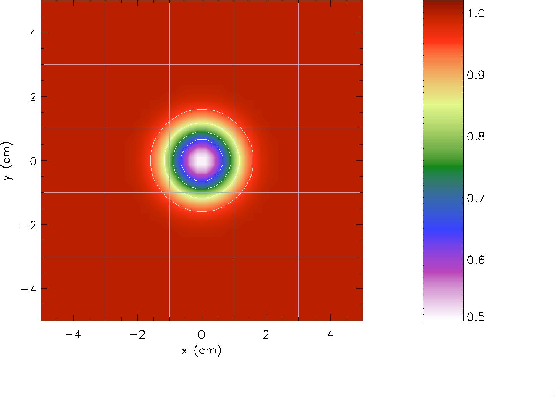
\includegraphics[width=5in]{IsentropicVortex1}}
\end{center}
\caption{\label{Fig:iv1} Density at $t=0.0$ for the isentropic vortex 
problem. Shown are the initial condition and the exact solution
at $t=10.0, 20.0, \ldots$.}
\end{figure}

A numerical simulation using the PPM scheme was run to illustrate
such errors. The simulation used the same grid shown in
\figref{Fig:iv1} with the same contour levels and color values. The
grid is intentionally coarse and the evolution time long to make
numerical errors visible.  The vortex is represented by
approximately 8 grid points in each coordinate direction and is
advected diagonally with respect to the grid.  At solution times of
$t=10, 20, \ldots$, \etc, the vortex should be back at its initial
location.

\figref{Fig:iv2} shows the solution at $t=50.0$; only slight
differences are observed. The density distribution is almost
radially symmetric, although the minimum density has risen to
$0.0537360$. Accumulating dispersion error is clearly visible at
$t=100.0$ (\figref{Fig:iv3}), and the minimum density is now
$0.601786$.
\begin{figure}
\begin{center}
{\leavevmode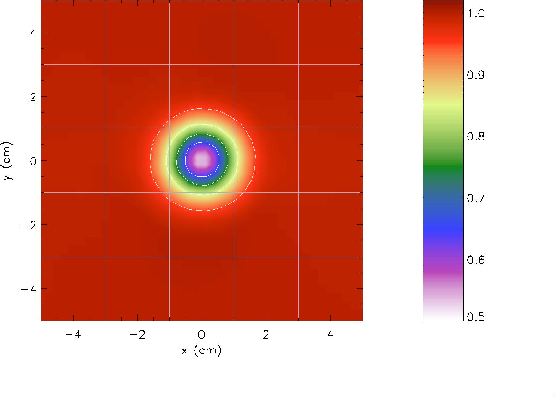
\includegraphics[width=5in]{IsentropicVortex2}}
\end{center}
\caption{\label{Fig:iv2} Density at $t=50.0$ for the isentropic
vortex problem.}
\end{figure}

\begin{figure}
\begin{center}
{\leavevmode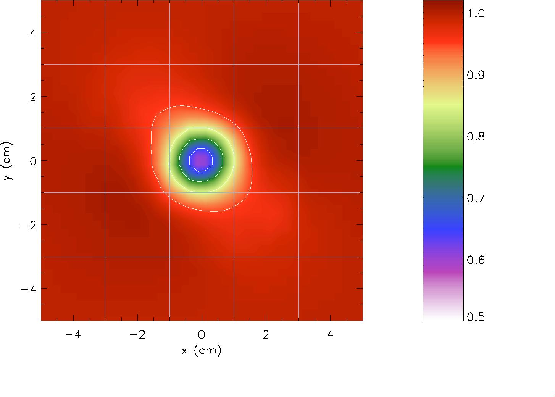
\includegraphics[width=5in]{IsentropicVortex3}}
\end{center}
\caption{\label{Fig:iv3} Density at $t=100.0$ for the isentropic
vortex problem.}
\end{figure}

\figref{Fig:iv4} shows the density near $y=0.0$ at three simulation
times. The black line shows the initial condition. The red line
corresponds to $t=50.0$ and the blue line to $t=100.0$. For the
later two times, the density is not radially symmetric. The lines
plotted are just representative profiles for those times, which give
an idea of the magnitude and character of the errors.
\begin{figure}
\begin{center}
{\leavevmode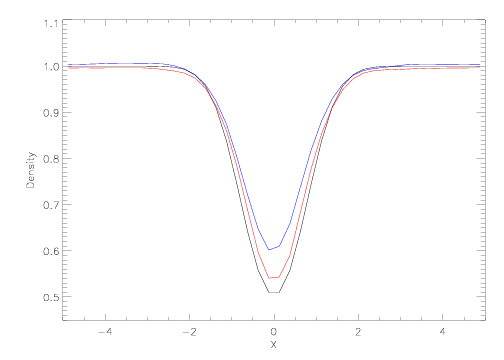
\includegraphics[width=5in]{IsentropicVortex4}}
\end{center}
\caption{\label{Fig:iv4} Representative density profiles for the isentropic
vortex near $y=0.0$ at $t=0.0$ (black), $t=50.0$ (red), and $t=100.0$ (blue).}
\end{figure}

 % This section was added by Lynn Reid from info provided by Alan Calder.
% she has several figures but cannot determine which one is which described below.
% hence this whole section is removed.
%
%% Then someone enable the section again. Then Klaus commented it out again
%% after talking to Anshu, since the figures are still not included. - KW

% \subsubsection{Isentropic Vortex with Particles}
% 
% The problem consists of an isentropic vortex either
% at rest relative to the center of the mesh or propagating across the
% mesh. The tracer particle verification tests with this problem consisted
% of propagating particles with the flow and measuring the error of the
% particle positions relative to the initial conditions. We note that
% measuring the error of the particle positions with the vortex evolving
% also measures the error in the vortex itself as it hydrodynamically
% evolves.
% 
% The isentropic vortex simulation domain as set up for these tests
% is a square, $-5.0 \mathrm{cm} \leq x, y \leq 5.0 \mathrm{cm}$.
% The ambient conditions are $u_{\infty}=1.0 cms $, $v_{\infty} = 1.0 cms $,
% and $T_{\infty} = 1.0 \mathrm{K}$.   The equations of \eqref{Eqn:isentropic_three} hold,
% with initial conditions as given before.
% The flow field is initialized by computing cell averages of the
% conserved variables: each average is approximated by averaging
% over $10^2$ subintervals in the cell. The simulations have periodic boundary
% conditions and time step is fixed.
% 
% The first test of the tracer particles was a consistency test between
% particles propagating in a static vortex and particles propagating in
% a vortex moving diagonally across the grid. \figref{fig:isen01}
% shows the initial velocity distribution for the stationary vortex. The
% moving vortex has an additional constant velocity added that moves the
% vortex diagonally across the grid. Also shown are points indicating the
% initial positions of three test particles. The particles were initially
% 0.2608, 0.7680, and 3.8732 cm from the center of the vortex. The metric
% for comparison in this test was the total velocity of each particle. The
% location of each particle determines its initial velocity, and ideally,
% the particles would maintain exactly the same total velocity over the
% course of the simulation.
% 
% \figref{fig:isen02} shows the velocity of the three test particles
% for both the static and moving vortex cases for 5 s. for a simulation on
% a $128 \times 128$ cell mesh. The velocity of the moving vortex particles
% has the constant translational velocity subtracted.  Also, the particles
% initially have zero velocity and obtain their velocity from the mesh at
% the first time step, and the initial zero velocities have been omitted
% from the plot for clarity. In the figure, the black lines indicate
% the the tracer particle velocities in the static vortex simulation,
% and the gray lines indicate the corrected tracer particle velocities
% in the moving vortex case.  The velocities show good agreement between
% the static and moving vortex simulations and also remain very close
% to constant during the course of the simulation.  In the static vortex
% case, maximum deviation of the radius of any particle reached only 0.3\%
% over the 5 s evolution.
% 
% The next series of tests consisted of resolution studies in space and time. In
% these tests, particles near the center of the vortex were propagated for one
% orbit of the vortex while measuring the radius of the orbit. Ideally, the radius
% of the orbit would remain constant. \figref{fig:isen03} plots the change in
% radius vs.\ time for tracer particles initially 0.261 cm from the center
% of the vortex in simulations on a $128 \times 128$ cell
% simulation mesh at decreasing time steps. The results show that while it
% remains relatively small, the error does not converge with decreasing time
% step.




%-------------------------------------------------------------------------------
\subsection{The double Mach reflection problem}
This numerical planar shock test problem introduced by Woodward and Colella (1984)
simulates an evolution of an unsteady planar shock
that is incident on an oblique surface. 
Initially, the incident planar shock begins to propagate
to the bottom surface at a $30^{\circ}$ angle with the shock Mach number of 10. 
Later, the solution to this problem produces a self-similar wave pattern that corresponds to the double Mach reflection.
Following many other numerical setups of this problem, 
we tilt the incident shock rather than the reflecting wall so as to avoid numerical complications in modeling
an oblique physical boundary. 

The initial setup involves a Mach 10 shock in air, $\gamma = 1.4$, on a rectangular 2D domain of size
$[0,4]\times[0,1]$. The reflecting wall is represented as the bottom surface of the domain, beginning at $x=1/6$.
The velocity normal to the incident shock in the post-shock region is 8.25, and the flow is at rest in the pre-shock region.
The undisturbed air ahead of the shock has a density of 1.4 and a pressure of 1. 
See the initial density profile in \figref{Fig:DMR_densityAMR_t0} resolved on 6 refinement AMR levels using {16$^2$}-cell block size.

The boundary condition on $0\le x \le 1/6$ at $y=0$ is fixed in time with the initial values so that the reflected shock
is attached to the bottom surface. We impose reflecting boundary condition (i.e., negating the $y$ velocity field $v$)
on the rest of the bottom surface. On the top surface of $y=1$, we allow the initial Mach 10 shock proceeds
exactly as a function of time in order that the numerical evolution follows the oblique shock propagation without any planar distortion.
At $x=0$, we impose a supersonic inflow boundary condition, and the outflow condition at $x=4$.

In later time, the solution develops to form two Mach stems and two contact discontinuities, 
as shown in \figref{Fig:DMR_density} the density at $t=2.5$ sec. Also shown 
in \figref{Fig:DMR_presContour} are 30 levels of contour lines of pressure, 
illustrating the evolved flow discontinuities at $t=2.5$ sec. We can also see that the numerical solution is 
smooth and non-oscillatory in the region bounded by the curved reflected shock, the bottom surface and
the second Mach stem (see more discussion in Woodward and Colella, 1984).


The 5th order WENO method in the unsplit hydrodynamics solver is used with a choice of hybrid Riemann solver which selectively adopts 
HLL only at strong shocks and HLLC otherwise.


\begin{figure}
\begin{center}
{\leavevmode\includegraphics[width=6in]{dmr_densAMRt0}}
\caption{\label{Fig:DMR_densityAMR_t0} The initial density at $t=0$ visualized with 6 levels of AMR block structures.
}
\end{center}
\end{figure}

\begin{figure}
\begin{center}
{\leavevmode\includegraphics[width=6in]{dmr_density}}
\caption{\label{Fig:DMR_density} Density profile at $t=2.5$. Two contact discontinuities are denoted as "CD",
along with two Mach stems, a curved reflected shock, and a jet formulation of the denser fluid along the bottom surface.
}
\end{center}
\end{figure}

\begin{figure}
\begin{center}
{\leavevmode\includegraphics[width=6in]{dmr_presContour}}
\caption{\label{Fig:DMR_presContour} The 30 levels of contour lines of pressure at $t=2.5$.
}
\end{center}
\end{figure}

\begin{table}
\caption{ \label{Tab:Mach parameters} Runtime parameters used with the
\code{double Mach reflection} test problem.}

\begin{center}
\begin{tabular}{lllp{3in}}
Variable   & Type      & Default   & Description\\
\hline
\code{sim\_rhoLeft}   & real      & 8     & Initial density to
the                          left of the shock
                         ($\rho_{\rm L}$)\\
\code{sim\_rhoRight}& real        & 1.4       & Initial density to the
                         right ($\rho_{\rm R}$)\\
\code{sim\_pLeft} & real      & 116.5     & Initial pressure to the
                         left ($p_{\rm L}$)\\
\code{sim\_pRight}    & real      & 1     & Initial pressure to the
                         right ($p_{\rm R}$)\\
\code{sim\_uLeft} & real      &     7.1447096  & Initial $x$-velocity
                         %(perpendicular to shock)
                         to the left ($u_{\rm L}$)\\
\code{sim\_uRight}    & real      & 0     & Initial $x$-velocity
                         %(perpendicular to shock)
                         to the right ($u_{\rm R}$)\\
\code{sim\_vLeft} & real      & -4.125     & Initial $y$-velocity
                         %(perpendicular to shock)
                         to the left ($v_{\rm L}$)\\
\code{sim\_vRight}    & real      & 0     & Initial $y$-velocity
                         %(perpendicular to shock)
                         to the right ($v_{\rm R}$)\\
                         
\code{sim\_xangle}  & real      & -30       & Angle made by shock
                         normal with the $x$-axis
                         (degrees)\\
\code{sim\_yangle}  & real      & 90        & Angle made by shock
                         normal with the $y$-axis
                         (degrees)\\
\code{sim\_posn}    & real      & 1/6      & Point of intersection between
                         the shock plane and the
                         $x$-axis\\
\hline
\end{tabular}
\end{center}

\end{table}

\vfill
\eject

%-------------------------------------------------------------------------------


\newpage
\subsection{Wind Tunnel With a Step}
\label{Sec:SimulationWindTunnel}
The problem of a wind tunnel containing a step, \code{WindTunnel} was first described by
Emery (1968), who used it to compare several hydrodynamical methods.
Woodward and Colella (1984)
later used it to compare several more advanced methods, including PPM.
Although it has no analytical solution, this problem is useful because
it exercises a code's ability to handle unsteady shock interactions
in multiple dimensions. It also provides an example of the use of Flash-X
to solve problems with irregular boundaries.

The problem uses a two-dimensional rectangular domain three units wide
and one unit high. Between $x=0.6$ and $x=3$ along the $x$-axis is a
step 0.2 units high. The step is treated as a reflecting boundary, as
are the lower and upper boundaries in the $y$-direction. For the right-hand
$x$-boundary, we use an outflow (zero gradient) boundary condition, while
on the left-hand side we use an inflow boundary. In the inflow boundary
cells, we set the density to $\rho_0$, the pressure to $p_0$, and the
velocity to $u_0$, with the latter directed parallel to the $x$-axis.
The domain itself is also initialized with these values.
We use
\begin{equation}
\rho_0 = 1.4, \qquad p_0 = 1, \qquad u_0 = 3\ , \qquad \gamma = 1.4,
\end{equation}
which corresponds to a Mach 3 flow. Because the outflow is supersonic
throughout the calculation, we do not expect reflections from the
right-hand boundary.

\begin{figure}
\begin{center}
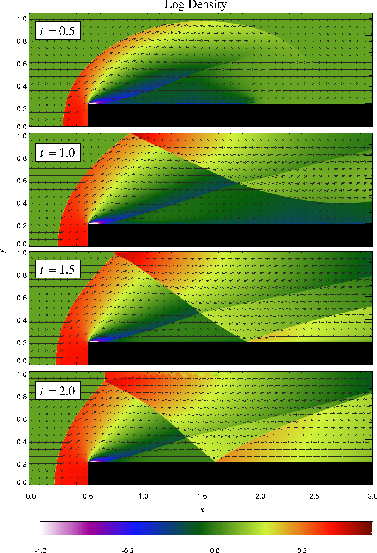
\includegraphics{WindTunnel_a} %, height=7in}
\caption{\label{Fig:Wind tunnel} Density and velocity in the Emery
wind tunnel test problem, as computed with Flash-X. A 2D grid with five
levels of refinement is used.
}
\end{center}
\end{figure}

\begin{figure}
\begin{center}
{\leavevmode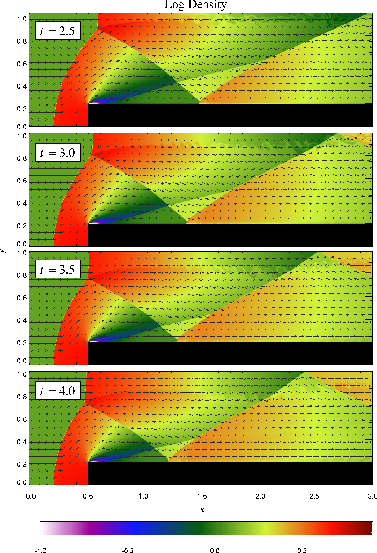
\includegraphics[height=7in]{WindTunnel_b}}
\end{center}
\addtocounter{figure}{-1}
\caption{\label{Fig:Wind tunnel (contd)} Density and velocity in the Emery
wind tunnel test problem (continued).
}
\end{figure}

The additional runtime parameters supplied with the
\code{WindTunnel} problem are listed in \tblref{Tab:Wind tunnel parameters}. 
This problem is configured to use the perfect-gas
equation of state (\code{Gamma}) with \rpi{Eos/gamma} set to 1.4. We
also set $\mbox{\rpi{Grid/xmax}}=3$, $\mbox{\rpi{Grid/ymax}}=1$, 
$\mbox{\rpi{Grid/Nblockx}}=15$, and
$\mbox{\rpi{Grid/Nblocky}}=5$ in order to create a grid with the correct
dimensions. The version of \api{Simulation/Simulation_defineDomain} supplied with this
problem 
removes all but the first three top-level blocks along the lower edge
of the grid to generate the step, and 
gives \code{REFLECTING} boundaries to the obstacle blocks. 
Finally, we
use \rpi{Grid/xl_boundary_type} \code{= "user"} (\code{USER\_DEFINED} condition) and
\rpi{Grid/xr\_boundary\_type} \code{= "outflow"} (\code{OUTFLOW} boundary) to instruct Flash-X to use
the correct boundary conditions in the $x$-direction. Boundaries in
the $y$-direction are reflecting (\code{REFLECTING}).

Until $t=12$, the flow is unsteady, exhibiting multiple shock
reflections and interactions between different types of
discontinuities. \figref{Fig:Wind tunnel} shows the evolution of
density and velocity between $t=0$ and $t=4$ (the period considered
by Woodward and Colella). Immediately, a shock forms directly in
front of the step and begins to move slowly away from it.
Simultaneously, the shock curves around the corner of the step,
extending farther downstream and growing in size until it strikes
the upper boundary just after $t=0.5$. The corner of the step
becomes a singular point, with a rarefaction fan connecting the
still gas just above the step to the shocked gas in front of it.
Entropy errors generated in the vicinity of this singular point
produce a numerical boundary layer about one cell thick along the
surface of the step. Woodward and Colella reduce this effect by
resetting the cells immediately behind the corner to conserve
entropy and the sum of enthalpy and specific kinetic energy through
the rarefaction. However, we are less interested here in reproducing
the exact solution than in verifying the code and examining the
behavior of such numerical effects as resolution is increased, so we
do not apply this additional boundary condition. The errors near the
corner result in a slight over-expansion of the gas there and a weak
oblique shock where this gas flows back toward the step. At all
resolutions we also see interactions between the numerical boundary
layer and the reflected shocks that appear later in the calculation.

The shock reaches the top wall at $t\approx 0.65$.  The point of
reflection begins at $x\approx 1.45$  and then moves to the left,
reaching $x\approx 0.95$ at $t=1$. As it moves, the angle between
the incident shock and the wall increases until $t=1.5$, at which
point it exceeds the maximum angle for regular reflection
($40^\circ$ for $\gamma=1.4$) and begins to form a Mach stem.
Meanwhile the reflected shock has itself reflected from the top of
the step, and here too the point of intersection moves leftward,
reaching $x\approx 1.65$ by $t=2$. The second reflection propagates
back toward the top of the grid, reaching it at $t=2.5$ and forming
a third reflection. By this time in low-resolution runs, we see a
second Mach stem forming at the shock reflection from the top of the
step; this results from the interaction of the shock with the
numerical boundary layer, which causes the angle of incidence to
increase faster than in the converged solution. \figref{Fig:Wind
tunnel comparison} compares the density field at $t=4$ as computed
by Flash-X using several different maximum levels of refinement. Note
that the size of the artificial Mach reflection diminishes as
resolution improves.

\begin{figure}
\begin{center}
{\leavevmode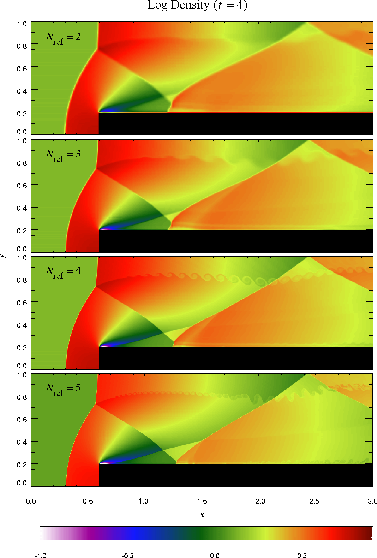
\includegraphics[height=7in]{WindTunnel_compare}}
\end{center}
\caption{\label{Fig:Wind tunnel comparison} Density at $t=4$ in the Emery
wind tunnel test problem, as computed with Flash-X using several different
levels of refinement.
}
\end{figure}

\begin{figure}
\begin{center}
{\leavevmode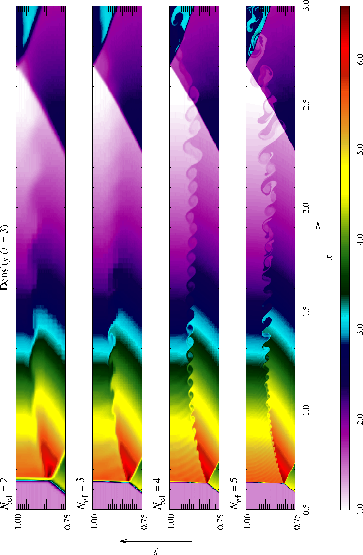
\includegraphics[height=6in,angle=-90]{WindTunnel_kh_detail}}
\end{center}
\caption{\label{Fig:Wind tunnel KH} Detail of the Kelvin-Helmholtz
instability seen at $t=3$ in the Emery
wind tunnel test problem for several different levels of refinement.
}
\end{figure}

The shear cell behind the first (``real'') Mach stem produces
another interesting numerical effect, visible at $t \ge 3$ ---
Kelvin-Helmholtz amplification of numerical errors generated at the
shock intersection. The waves thus generated propagate downstream
and are refracted by the second and third reflected shocks. This
effect is also seen in the calculations of Woodward and Colella,
although their resolution was too low to capture the detailed eddy
structure we see. \figref{Fig:Wind tunnel KH} shows the detail of
this structure at $t=3$ on grids with several different levels of
refinement. The effect does not disappear with increasing
resolution, for three reasons. First, the instability amplifies
numerical errors generated at the shock intersection, no matter how
small. Second, PPM captures the slowly moving, nearly vertical Mach
stem with only 1--2 cells on any grid, so as it moves from one
column of cells to the next, artificial kinks form near the
intersection, providing the seed perturbation for the instability.
Third, the effect of numerical viscosity, which can diffuse away
instabilities on course grids, is greatly reduced at high
resolution. This effect can be reduced by using a small amount of
extra dissipation to smear out the shock, as discussed by Colella
and Woodward (1984). This tendency of physical instabilities to
amplify numerical noise vividly demonstrates the need to exercise
caution when interpreting features in supposedly converged
calculations.


\begin{table}

\caption{Runtime parameters used with the
\code{WindTunnel} test problem. }
\label{Tab:Wind tunnel parameters}
\begin{center}
\begin{tabular}{lllp{3in}}
Variable    & Type      & Default   & Description\\
\hline
\code{sim\_pAmbient}  & real   & 1 & Ambient pressure ($p_0$)\\
\code{sim\_rhoAmbient}& real   & 1.4   & Ambient density ($\rho_0$)\\
\code{sim\_windVel}   & real    & 3 & Inflow velocity ($u_0$)\\
\hline
\end{tabular}
\end{center}

\end{table}
Finally, we note that in high-resolution runs with Flash-X, we also see
some Kelvin-Helmholtz roll up at the numerical boundary layer along the
top of the step. This is not present in Woodward and Colella's calculation,
presumably because their grid resolution was lower (corresponding to two
levels of refinement for us) and because of their special
treatment of the singular point.


\subsection{Driven Turbulence \code{StirTurb}}
\label{Sec:SimulationStirturb}
The driven turbulence problem \code{StirTurb} simulates homogeneous, isotropic and
weakly-compressible turbulence. Because theories of turbulence
generally assume a steady state, and because turbulence is inherently
a  dissipative phenomenon, the fluid must be driven to sustain a steady-state. 
This driving must be done carefully in order to avoid introducing 
artifacts into the turbulent flow.  We use a relatively sophisticated
stochastic driving method originally introduced by Eswaran \& Pope (1988).
The initial conditions sets up a homogeneous background. The resolution used for
this test run was $32^3$, and the boundary conditions were
periodic. The \tblref{Tab:Driventurb parameters} shows values
the runtime parameters values to control the amount of driving, and
the Figures \figref{Fig:stirturb_dens} and \figref{Fig:stirturb_velx} show
the density and x velocity 
profile of an xy plane in the center of the domain.
\begin{table}

\caption{ Runtime parameters used with the
\code{Driven Turbulence} test problem.}
\label{Tab:Driventurb parameters} 
\begin{center}
\begin{tabular}{lllp{3in}}
Variable    & Type      & Value   & Description\\
\hline
\code{st\_stirmax}  & real   & 25.1327 & maximum stirring wavenumber\\
\code{st\_stirmin}& real   & 6.2832   & minimum stirring wavenumber\\
\code{st\_energy}      & real    & 5.E-6 & energy input per mode\\
\code{st\_decay}      & real    & 0.5 & correlation time for driving\\
\code{st\_freq}      & integer    & 1 & frequency of stirring\\
\hline
\end{tabular}
\end{center}
\end{table}

\begin{figure}
\begin{center}
{\leavevmode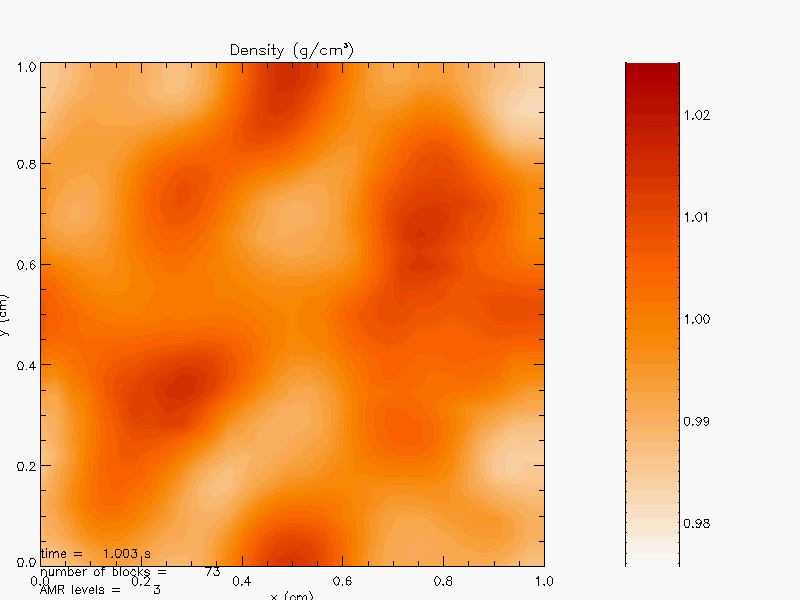
\includegraphics[width=3.5in]{StirTurb_dens}}
\end{center}
\caption{\label{Fig:stirturb_dens} Density profile for the \code{StirTurb}
driven turbulence problem. }
\end{figure}

\begin{figure}
\begin{center}
{\leavevmode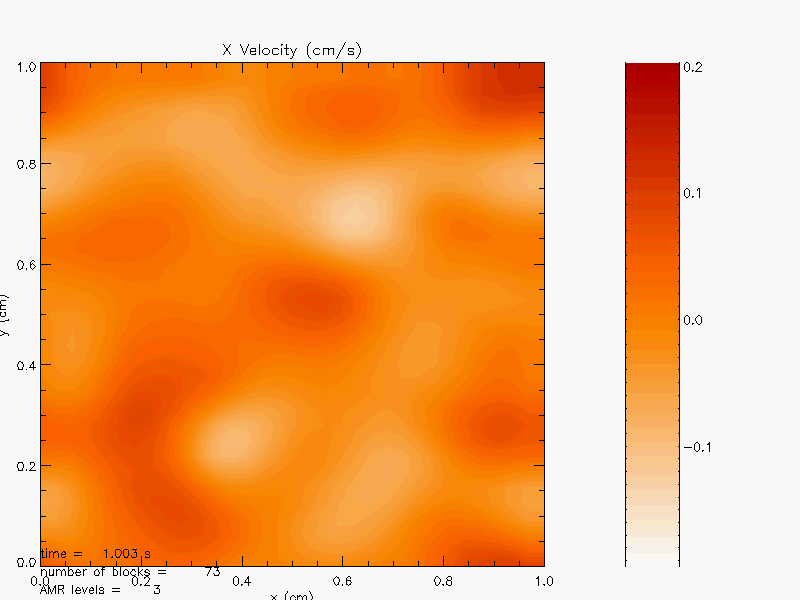
\includegraphics[width=3.5in]{StirTurb_velx}}
\end{center}
\caption{\label{Fig:stirturb_velx} velocity along X dimension for the \code{StirTurb}
driven turbulence problem. }
\end{figure}

%-----------------------------------------------------------------------------------------


%-----------------------------------------------------------------------------------------
\newpage
\subsection{Flow Interactions with Stationary Rigid Body}
The stationary rigid body is only implemented and tested in the unsplit hydro solver \secref{Sec:unsplit hydro algorithm}. 
It is possible that the unsplit staggered mesh MHD solver \secref{Sec:usm_algorithm} can support the rigid body but we have not
tested yet.

\subsubsection{NACA Airfoil}
\label{Sec:SimulationFlatPlate}
Flow simulations over a series of NACA airfoils (or a simple flat plate) can be obtained using the 
implementation of a stationary rigid body in the unsplit hydro solver described in \secref{Sec:StationaryRigidBody}.
In this example, the cambered NACA2412 airfoil is initialized 
with positive unity values indicating the part of the domain that
belongs to a stationary rigid body. The rest of the domain is assigned negative unity values to indicate it as
a flow region for the unsplit hydro solver.
At the surface of the rigid body, a reflecting boundary condition is applied in order to represent the fact that there is
no flow penetrating the rigid object.

Plots in \figref{Fig:NACA2412_Mach0.65_mach} -- \figref{Fig:NACA2412_Mach1.2_pres} illusrate 
Mach number and pressure plots over the airfoil with the three different initial Mach numbers, 0.65, 0.95 and 1.2 at $t=1.8.$ 
By this time, the flow conditions have reached their steady states. For Mach number = 0.65, the critical Mach number has not yet
been obtained and the flow over the airfoil is all subsonic as shown in \figref{Fig:NACA2412_Mach0.65_mach}. Since the airfoil is
asymmetric and cambered, we see there are pressure gradients across the top and bottom surfaces 
even at zero angle of attack in \figref{Fig:NACA2412_Mach0.65_pres}. 
These pressure gradients (higher pressure at the bottom than the top) generate a lift force 
by which an airplane can fly defying gravity. 

At Mach number reaching 0.95 as shown in \figref{Fig:NACA2412_Mach0.95_mach} there are local points 
that are supersonic. This indicates that the critical Mach number for the airfoil is between 
0.65 and 0.95. In fact, one can show that the critical Mach number is around 0.7 for the NACA2412 airfoil.
We see that there is a development of a bow shock formation in front of the airfoil. 
A formation of a subsonic region between the bow shock
and the nose of the airfoil is visible in the Mach number plot. Inside the bow shock, a sonic line at which
the local flow speed becomes the sound speed makes an oval shape together with the bow shock.   
In both the Mach number and pressure plots, a strong wake forms starting from 
the top and bottom of the surfaces near the trailing edge.
The wake is hardly visible for Mach number 0.65 in \figref{Fig:NACA2412_Mach0.65_mach} and \figref{Fig:NACA2412_Mach0.65_pres}.
Normal shock waves have formed steming from the trailing edge as seen in \figref{Fig:NACA2412_Mach0.95_mach} and
\figref{Fig:NACA2412_Mach0.95_pres}.

At Mach number 1.2 the flow becomes supersonic everywhere. 
In this case, the shape of the bow shock becomes narrower and there are much larger supersonic pockets developed on the top and bottom
surfaces with a smaller subsonic region between the bow shock and the nose region.

\begin{figure}[ht]
\begin{center}
\subfigure[a]{\label{Fig:NACA2412_Mach0.65_mach}
  \includegraphics[width=3.0in]{naca2412_mach0p65_hdf5_chk_mach0006}
}
\subfigure[b]{\label{Fig:NACA2412_Mach0.65_pres}
 \includegraphics[width=3.0in]{naca2412_mach0p65_hdf5_chk_pres0006}
}
\caption{
  NACA2412 in Mach number 0.65 flow at 0 degree angle of attack problem at $t=1.8$ (a) Mach number (b) Pressure
}
\end{center}
\end{figure}



\begin{figure}[ht]
\begin{center}
\subfigure[a]{\label{Fig:NACA2412_Mach0.95_mach}
 \includegraphics[width=3.0in]{naca2412_mach0p95_hdf5_chk_mach0006}
}
\subfigure[b]{\label{Fig:NACA2412_Mach0.95_pres}
 \includegraphics[width=3.0in]{naca2412_mach0p95_hdf5_chk_pres0006}
}
\caption{
  NACA2412 in Mach number 0.95 flow at 0 degree angle of attack problem at $t=1.8$ (a) Mach number (b) Pressure
}
\end{center}
\end{figure}



\begin{figure}[ht]
\begin{center}
\subfigure[a]{\label{Fig:NACA2412_Mach1.2_mach}
 \includegraphics[width=3.0in]{naca2412_mach1p2_hdf5_chk_mach0006}
}
\subfigure[b]{\label{Fig:NACA2412_Mach1.2_pres}
 \includegraphics[width=3.0in]{naca2412_mach1p2_hdf5_chk_pres0006}
}
\caption{
  NACA2412 in Mach number 1.2 flow at 0 degree angle of attack problem at $t=1.8$ (a) Mach number (b) Pressure
}
\end{center}
\end{figure}




%\begin{figure}
%\begin{center}
%{\leavevmode\includegraphics[width=5in]{rhd_riemann2Dhdf5_chk_dens0008}}
%\end{center}
%\caption{\label{Fig:NACA0015_pres} Pressure plot for the NACA2412 airfoil at Mach number 1.2 and angle of attact 6 degrees at t=2.0.
%}
%\end{figure}

%\begin{figure}
%\begin{center}
%{\leavevmode\includegraphics[width=5in]{rhd_riemann2Dhdf5_chk_dens0008}}
%\end{center}
%\caption{\label{Fig:NACA2412_pres} Pressure plot for the NACA2412 airfoil at Mach number 1.2 and angle of attact 6 degrees at t=2.0.
%}
%\end{figure}

\subsubsection{Solid Objects in Sedov Explosion}
\label{Sec:SimulationSedovChamber}
Another problem for testing a stationary rigid body in a simulation is to consider the Sedov-like explosion in a chamber surrounded by
a solid wall with holes The wall is shown as red blocks with white boundry in \figref{Fig:sedovChamber_t0} and \figref{Fig:sedovChamber_t0p1}. 
The simulation was done on a uniform Cartesian grid with 300 cells on each direction. Three holes in the wall
subdivide it into four different stationary solid bodies in a square computational domain $[0,1.5] \times [0,1.5]$. The explosion goes
off at the origin and generate shock waves inside the chamber. In later time, when the shock waves pass though the three holes in the wall, 
turbulence effects are triggered from the interaction between the fluid and the wall and enhance vortical fluid motions.

One important thing in this problem is to keep the given symmetry throughout the simulation. The flow symmetry across the diagonal direction
is well preseved in \figref{Fig:sedovChamber_t0} and \figref{Fig:sedovChamber_t0p1}.

\begin{figure}[t]
\begin{center}
\subfigure[a]{\label{Fig:sedovChamber_t0}
 \includegraphics[width=3.0in]{fl-sedovch-flash-1}
}
\subfigure[b]{\label{Fig:sedovChamber_t0p1}
 \includegraphics[width=3.0in]{fl-sedovch-flash-5}
}
\caption{
  The Sedov explosion in a chamber surrounded by a wall with holes. (a) Density plot at $t=0.0$ sec. (b) Denstiy plot at $t=0.1$ sec.
}
\end{center}
\end{figure}

%-----------------------------------------------------------------------------------------
\newpage
\section{Magnetohydrodynamics Test Problems}
The magnetohydrodynamics (MHD) test problems provided in this release can be found in
\code{source/\-Simulation/\-SimulationMain/\-magnetoHD/}. In order to set up an MHD problem,
users need to specify the \code{magnetoHD} path in a setup script. For instance, the \code{BrioWu}
problem can be configured by typing \code{./setup magnetoHD/BrioWu -auto -1d}.
\subsection{Brio-Wu MHD Shock Tube}
\label{Sec:SimulationBrioWu}

The Brio-Wu MHD shock tube problem (Brio and Wu, 1988),
\code{magnetoHD/BrioWu}, is a
coplanar magnetohydrodynamic counterpart of the hydrodynamic Sod
problem (\secref{Sec:SimulationSod}). The initial left
and right states are given by $\rho_l=1$, $u_l=v_l=0$, $p_l=1$,
$(B_y)_l=1$; and $\rho_r=0.125$, $u_r=v_r=0$, $p_r=0.1$,
$(B_y)_r=-1$. In addition, $B_x=0.75$ and $\gamma=2$. This is a good
problem to test wave properties of a particular MHD solver, because
it involves two fast rarefaction waves, a slow compound wave, a
contact discontinuity and a slow shock wave.

The conventional 800 point solution to this problem computed with
Flash-X is presented in \figref{Fig:bw_density},
\figref{Fig:bw_pressure}, \figref{Fig:magnetic},
\figref{Fig:bw_velx}, and \figref{Fig:bw_vely} . The figures show the
distribution of density, normal and tangential velocity components,
tangential magnetic field component and pressure at $t=0.1$ (in
non-dimensional units). As can be seen, the code accurately and
sharply resolves all waves present in the solution. There is a small
undershoot in the solution at $x\approx0.44$, which results from a
discontinuity-enhancing monotonized centered gradient limiting
function (LeVeque 1997). This undershoot can be easily removed if a
less aggressive limiter, {\it e.g.} a minmod or a van Leer limiter,
is used instead. This, however, will degrade the sharp resolution of
other discontinuities.

The directionally splitting \code{8Wave} MHD solver
with a second-order MUSCL-Hancock scheme (setup with \code{+8wave}) was used 
for the results shown in this simulation.
The \code{StaggeredMesh} MHD solver (setup with \code{+usm}) can also be used
for this Brio-Wu problem in one- and two-dimensions.
However, in the latter case, the \code{StaggeredMesh}
solver only supports non-rotated setups for which
a shock normal is parallel to the $x$-axis that
initially intersects that axis
at $x=0.5$ (halfway across a box with unit dimensions).
This limitation occurs in the \code{StaggeredMesh}
scheme because the currently released version of
the Flash-X code does not truly support physically
correct boundary conditions for this rotated shock
geometry.


\begin{figure}[!ht]
\begin{center}
{\leavevmode\includegraphics[width=2.5in]{BrioWu_dens}}
\end{center}
\caption{\label{Fig:bw_density} Density profile for the
Brio-Wu shock tube problem. }
\end{figure}

\begin{figure}[!ht]
\begin{center}
{\leavevmode\includegraphics[width=2.5in]{BrioWu_pres}}
\end{center}
\caption{\label{Fig:bw_pressure} Pressure profile for the
Brio-Wu shock tube problem. }
\end{figure}

\begin{figure}[!ht]
\begin{center}
{\leavevmode\includegraphics[width=2.5in]{BrioWu_magy}}
\end{center}
\caption{\label{Fig:magnetic} Tangential magnetic
field profile for the Brio-Wu shock tube problem.}
\end{figure}

\begin{figure}[!ht]
\begin{center}
{\leavevmode\includegraphics[width=2.5in]{BrioWu_velx}}
\end{center}
\caption{\label{Fig:bw_velx} Normal velocity profile
for the Brio-Wu shock tube problem.
}
\end{figure}

\begin{figure}[!ht]
\begin{center}
{\leavevmode\includegraphics[width=2.5in]{BrioWu_vely}}
\end{center}
\caption{\label{Fig:bw_vely} Tangential velocity profile
for the Brio-Wu shock tube problem.
}
\end{figure}

%\clearpage
%\vfill
%\eject
\subsubsection{Slowly moving shocks (SMS) issues in the Brio-Wu problem}
%begin{latexonly}
\makeUsMath
%end{latexonly}

Figure ~\ref{fig:BrioWu_standardPPM_a} clearly demonstrates that the
conventional PPM reconstruction method fails to preserve
monotonicities, shedding oscillations  especially in the plateau
near strong discontinuities such as the contact and right
going slow MHD shock. In Fig.~\ref{fig:BrioWu_standardPPM_b}, Mach
numbers are plotted with varying strengths of the transverse field
$B_y$. The oscillations increase with an increase of $B_y$;
the reason being that stronger $B_y$ introduces more transverse effect
that resists shock propagation in the $x$ direction causing the
shock to move slowly. This effect is clearly seen in the locations of
the shock fronts (right going slow MHD shocks in this case), which
remain closer to the initial location $x=0.5$ when $B_y$ is
stronger. %For $B_y=1$, $S/\lambda_{\mbox{max}}$ reaches 0.136,
%which is in a range of quasi-steady SMS.
%In this paper we do not consider values of
%$S/\lambda_{\mbox{max}}<0.1$ because at those values even the PLM method
%begins to oscillate.


\begin{figure}[!htbp]
\begin{center}
{\leavevmode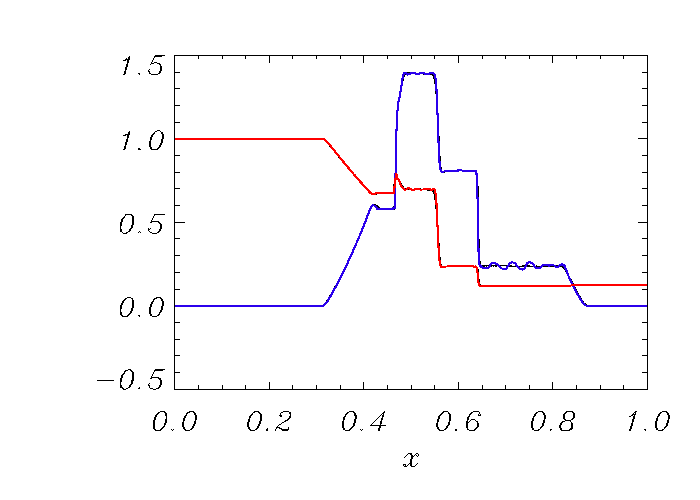
\includegraphics[width=4in]{Lee_fig7}}
\end{center}
\caption{\label{fig:BrioWu_standardPPM_a} Density (thick red) and Mach number (thick blue) at $t=0.1$ of the Brio-Wu test with the conventional PPM's MC limiter. Thin black curves represent
reference solutions using the PLM of MUSCL-Hancock scheme. Severe numerical oscillations are evident in the solution using the conventional PPM reconstruction on 400 grid points.
}
\end{figure}

\begin{figure}[!htbp]
\begin{center}
{\leavevmode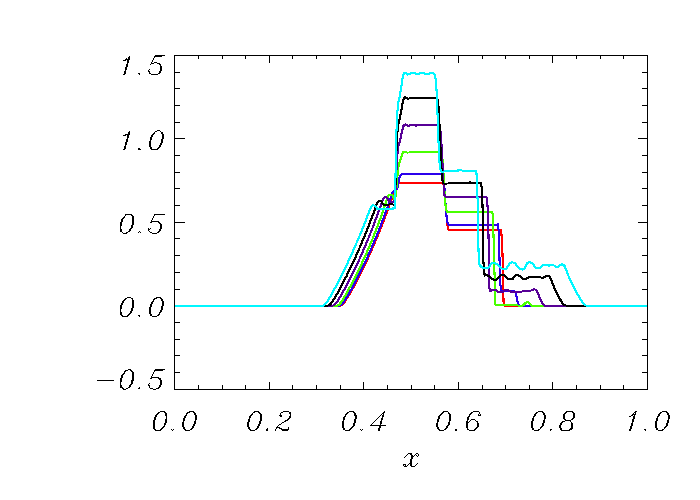
\includegraphics[width=4in]{Lee_fig8}}
\end{center}
\caption{\label{fig:BrioWu_standardPPM_b} Mach numbers at $t=0.1$ with varying $B_y$ from 0 to 1 with the conventional PPM's MC limiter. Curves in red, blue, green, purple, black, and cyan
represent $B_y=0, 0.2, 0.4, 0.6, 0.8,$ and $1$, respectively. Severe numerical oscillations are evident in the solution using the conventional PPM reconstruction on 400 grid points.
}
\end{figure}

%\begin{figure}[!htbp]
%\centerline{
%{\subfigure[Density (thick red) and Mach number (thick blue) at $t=0.1$ of the Brio-Wu test with the conventional PPM's MC limiter. Thin black curves represent
%reference solutions using the PLM of MUSCL-Hancock scheme.]
%{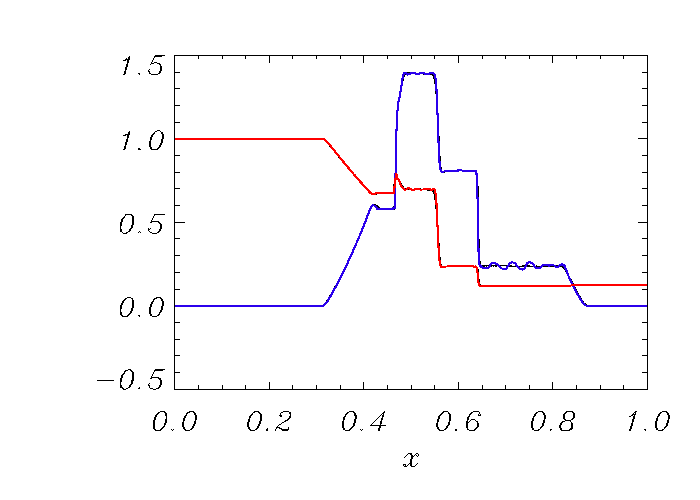
\includegraphics[width=2.6in,height=2.0in]{Lee_fig7}}}
%{\subfigure[Mach numbers at $t=0.1$ with varying $B_y$ from 0 to 1 with the conventional PPM's MC limiter. Curves in red, blue, green, purple, black, and cyan
%represent $B_y=0, 0.2, 0.4, 0.6, 0.8,$ and $1$, respectively.]
%{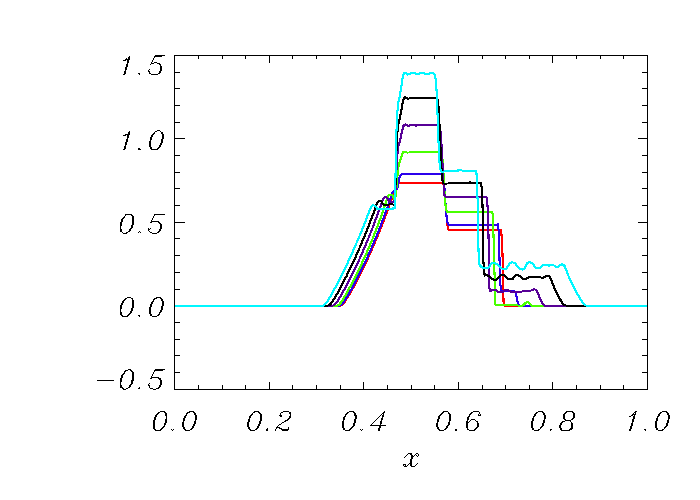
\includegraphics[width=2.6in,height=2.0in]{Lee_fig8}}}
%}
%\caption{Severe numerical oscillations are evident in the solution using the conventional PPM reconstruction on 400 grid points.}
%%The reference solution using PLM doesn't suffer from such oscillations.}
%\label{fig:BrioWu_standardPPM}
%%{\vskip-0.1in}
%\end{figure}

%begin{latexonly}
\makeUsNormal
%end{latexonly}

Results from using the upwind biased slope limiter for PPM are
illustrated in Figures ~\ref{fig:BrioWu_upwindPPM3} -- \ref{fig:BrioWu_upwindPPM6} .  The oscillation
shedding found in the conventional PPM  (e.g., Fig.~{\ref{fig:BrioWu_standardPPM_a}}) are significantly
reduced in both density, and Mach number profiles. 
The overall qualitative solution behavior of using the upwind PPM approach, shown in 
Fig.~\ref{fig:BrioWu_upwindPPM3}, 
is very much similar to those from the 5th order WENO method as illustrated in
Fig.~\ref{fig:BrioWu_upwindPPM4}.
As shown in the closeup views in Fig. ~\ref{fig:BrioWu_upwindPPM5} and  ~\ref{fig:BrioWu_upwindPPM6}, 
the solutions with the upwind PPM slope limiter (blue curves) outperforms 
the conventional PPM method (red curves), and compares well with the WENO scheme (green curves). 
In fact, the upwind approach shows the most flat
density plateau of all methods. Note that the SMS issue can be observed regardless of
the choice of Riemann solvers and the dissipation mechanism in PPM (e.g., even with flattening on).
400 grid points were used.
%Similar to our experience with Flash-X's
%\citep{dubey2009,Fryxell2000} PPM implementation, the oscillatory
%behavior can be seen with other HRSC codes such as ATHENA
%~\citep{StoneGardinerEtAlAthena2008} and PLUTO
%~\citep{MignonePluto2007}, regardless of the  choice of Riemann
%solvers (see ~\citep{LeePPMUpwind2010}). 

\begin{figure}[!htbp]
\begin{center}
{\leavevmode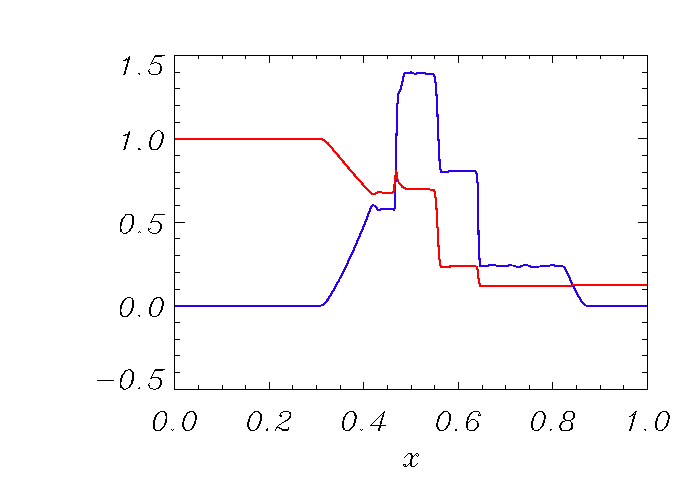
\includegraphics[width=4in]{Lee_fig3}}
\end{center}
\caption{\label{fig:BrioWu_upwindPPM3} Density (red) and Mach number (blue) at $t=0.1$ of the Brio-Wu test  using the upwind biased PPM limiter.
}
\end{figure}

\begin{figure}[!htbp]
\begin{center}
{\leavevmode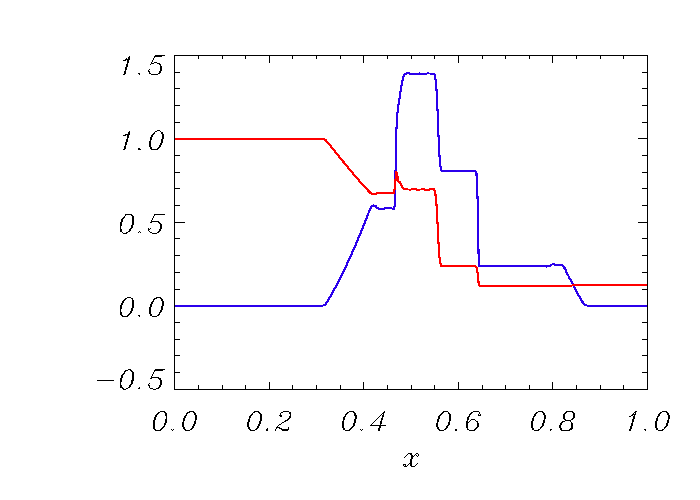
\includegraphics[width=4in]{Lee_fig4}}
\end{center}
\caption{\label{fig:BrioWu_upwindPPM4} Density (red) and Mach number (blue) at $t=0.1$ of the Brio-Wu test  using the 5th order WENO scheme.
}
\end{figure}

\begin{figure}[!htbp]
\begin{center}
{\leavevmode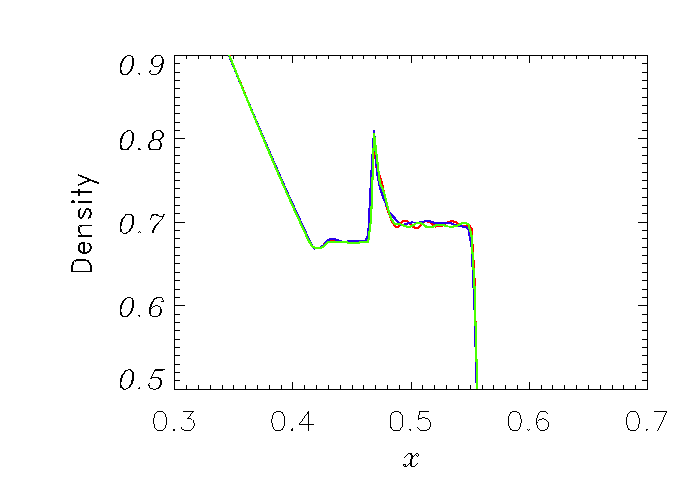
\includegraphics[width=4in]{Lee_fig5}}
\end{center}
\caption{\label{fig:BrioWu_upwindPPM5} Density closeup at $t=0.1$ of the Brio-Wu test. 
The conventional PPM in red curve, the upwind PPM in blue curve, and the WENO scheme in green curve.
}
\end{figure}

\begin{figure}[!htbp]
\begin{center}
{\leavevmode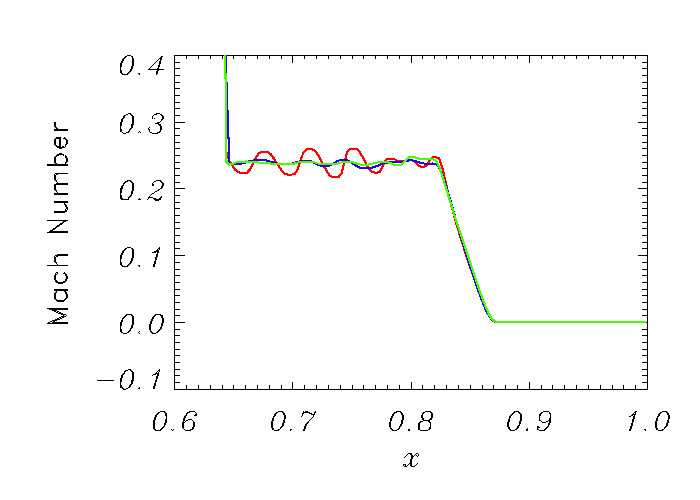
\includegraphics[width=4in]{Lee_fig6}}
\end{center}
\caption{\label{fig:BrioWu_upwindPPM6} Mach number closeup at $t=0.1$ of the Brio-Wu test.
The conventional PPM in red curve, the upwind PPM in blue curve, and the WENO scheme in green curve.
}
\end{figure}




%{\vskip-0.3in}
%\begin{figure}[!htbp]
%\centerline{
%{\subfigure[Density (red) and Mach number (blue) at $t=0.1$ of the Brio-Wu test  using the upwind biased PPM limiter.]
%{\includegraphics[width=2.6in,height=2.0in]{Lee_fig3}}}
%{\subfigure[Density (red) and Mach number (blue) at $t=0.1$ of the Brio-Wu test  using the 5th order WENO scheme.]
%{\includegraphics[width=2.6in,height=2.0in]{Lee_fig4}}}
%}
%\centerline{
%{\subfigure[Density closeup at $t=0.1$ of the Brio-Wu test.]
%{\includegraphics[width=2.6in,height=2.0in]{Lee_fig5}}}
%{\subfigure[Mach number closeup at $t=0.1$ of the Brio-Wu test.]
%{\includegraphics[width=2.6in,height=2.0in]{Lee_fig6}}}
%}%{\vskip-0.1in}
%\caption{Oscillations in density and Mach number are significantly reduced by using the upwind biased PPM limiter. The overall quality of
%the solution using the upwind PPM scheme (blue curves)
%compares very well with the 5th order WENO scheme solution (green curves). The conventional PPM scheme is represented in red curves.
%400 grid points were used.}
%\label{fig:BrioWu_upwindPPM}
%\end{figure}

%===============================================================================
\subsection{Orszag-Tang MHD Vortex}
\label{Sec:SimulationOrszagTang}

The Orszag-Tang MHD vortex problem (Orszag and Tang, 1979),
\code{magnetoHD/OrszagTang}, is a simple
two-dimensional problem that has become a classic test for MHD codes.
In this problem a simple, non-random initial condition is imposed at
time $t=0$
\begin{equation}
  {\bf V} = V_0\left(-\sin(2\pi y),\sin(2\pi x), 0\right),\mbox{~~~}
  {\bf B} = B_0\left(-\sin(2\pi y),\sin(4\pi x), 0\right),\mbox{~~~}
  (x,y)=\in[0,1]^2,
\end{equation}
where $B_0$ is chosen so that the ratio of the gas pressure to the RMS
magnetic pressure is equal to $2\gamma$. In this setup the initial
density, the speed of sound and $V_0$ are set to unity; therefore,
the initial pressure $p_0=1/\gamma$ and $B_0=1/\gamma$.

As the evolution time increases, the vortex flow pattern becomes
increasingly complicated due to the nonlinear interactions of waves.
A highly resolved simulation of this problem should produce
two-dimensional MHD turbulence. \figref{Fig:orszag_tang_density} and
\figref{Fig:orszag_tang_magfield} shows density and magnetic field
contours at $t=0.5$. As one can observe, the flow pattern at this
time is already quite complicated. A number of strong waves have
formed and passed through each other, creating turbulent flow
features at all spatial scales.

The results were obtained using the directionally splitting
\code{8Wave} MHD solver for this Orszag-Tang problem.

\begin{figure}[!ht]
\begin{center}
{\leavevmode\includegraphics[width=3.5in]{OrszagTang_dens}}
\end{center}
\caption{\label{Fig:orszag_tang_density} Density contours in the
Oszag-Tang MHD vortex problem at $t=0.5$. }
\end{figure}

\begin{figure}[!ht]
\begin{center}
{\leavevmode\includegraphics[width=3.5in]{OrszagTang_magf}}
\end{center}
\caption{\label{Fig:orszag_tang_magfield} Magnetic field contours
in the Oszag-Tang MHD vortex problem at $t=0.5$. }
\end{figure}
%\clearpage
%\vfill
%\eject
The 3D version are also shown in the below solved using the unsplit staggered mesh MHD solver. 

\begin{figure}[!ht]
\begin{center}
\subfigure[a]{\label{Fig:3D_OrszagTant_t0p2}
 \includegraphics[width=3.0in]{ot_dens_t0p2}
}
\subfigure[b]{\label{Fig:3D_OrszagTant_t0p5}
 \includegraphics[width=3.0in]{ot_dens_t0p5}
}
\subfigure[c]{\label{Fig:3D_OrszagTant_t0p7}
 \includegraphics[width=3.0in]{ot_dens_t0p7}
}
\subfigure[d]{\label{Fig:3D_OrszagTant_t1p0}
 \includegraphics[width=3.0in]{ot_dens_t1p0}
}
\caption{
  Density plots of a 3D version of the Orszag-Tang problem on a $128^3$ uniform grid resolution. (a) Density at $t=0.2$ (b) Density at $t=0.5$
 (c) Density at $t=0.7$ (d) Density at $t=1.0$.  
}
\end{center}
\end{figure}




%===============================================================================
\clearpage
\subsection{Magnetized Accretion Torus}
\label{Sec:SimulationAccretionTorus}

The magnetized accretion torus problem is based on the global magneto-rotational instability (MRI)
simulations of Hawley (2000). It can be found under \code{magnetoHD/Torus}.
We consider a magnetized torus of constant angular
momentum ($\Omega\propto r^{-2}$), inside a normalized Paczy\'nsky-Wiita pseudo-Newtonean
gravitational potential (Paczy\'nsky\&Wiita, 1980) of the form $\Phi=-1/(R-1)$, where
$R=\sqrt{r^2+z^2}$.

The cylindrical computational domain, with lengths normalized at $r_0$, 
extends from 1.5 $r_0$ to 15.5 $r_0$ in the radial direction and from -7 $r_0$
to 7 $r_0$ in the $z$ direction. For this specific simulation we use seven levels of
refinement, linear reconstruction with vanLeer limiter and the HLLC Riemann solver.  
The boundary conditions are set to outflow, except for
the leftmost side where a diode-like condition is applied.

Assuming an adiabatic equation of state, the initial density profile of the torus is given by
%
\begin{equation}
\DS \frac{\Gamma P}{(\Gamma-1)\rho} = C - \Phi -\frac{l_K^2}{2r^2},
\end{equation}
%
where the specific heats ratio is $\Gamma=5/3$, $l_K$ is the Keplerian
angular momentum at the pressure maximum ($r_{Pmax}=4.7 r_0$) and C is an
integration constant that specifies the outer surface of the torus,
given its inner radius ($r_{in}=3\,r_0$). The initial poloidal magnetic field 
is computed using the $\phi$ component of the vector potential,
$A_{\phi} \propto \textrm{max}(\rho-5,\,0)$, and normalized so as the initial
minimum value of the plasma $\beta=2P/{\bf B}^2$ is equal to $10^2$. The resulting field
follows the contours of density, i.e. torus-like nested loops, and is embedded
well within the torus.

We allow the system to evolve for $t=150\,t_0$. The torus is MRI unstable and
after approximately one revolution accretion sets in. The strong shear generates
an azimuthal field component and the angular momentum is redistributed. 
Due to the instability, fillamentary structures form at the torus surface
that account for its rich morphology (\figref{Fig:accretiontorus}).
These results can be promtly compared to those in Hawley (2000) and
Mignone et al. (2007).
%
\begin{figure}[!ht]
\begin{center}
\leavevmode\includegraphics[width=6.0in]{torus_composite}
\end{center}
\caption{\label{Fig:accretiontorus} Left: 3D rendering of the axisymmetric
torus evolution. Right: Density logarithm of the magnetized accretion torus
after 150 $t_0$. Superposed are the AMR levels and the mesh.}
\end{figure}
%

%===============================================================================
\clearpage
\subsection{Magnetized Noh Z-pinch}
\label{Sec:MagnetizedNoh}

In this test we consider the magnetized version of the classical Noh problem (Noh, 1987).
It consists of a cylindrically symmetric implosion of a pressure-less gas: the gas
stagnates at the symmetry axis and creates an outward moving accretion shock which
propagates at a constant velocity. The self-similar analytic solution of this problem
has been widely used as benchmark test for hydrodynamic codes, especially those targeting
implosion.

Recently, Velikovich et al. (2012) have extended the original test problem to include
an embedded azimuthal magnetic field, in accordance with the Z-pinch physics.
In their study, they present a family of exact analytic solutions for which the
values of primitive variables are finite everywhere, providing an excellent benchmark
for Z-pinch and general MHD codes.

We perform this test in both cartesian and cylindrical geometries. The tests
can be found respectively in \code{magnetoHD/Noh} and \code{magnetoHD/NohCylindrical}.
For brevity we describe only the cylindrical initialization. The cartesian can be
easily recovered by projecting the solution onto the X-Y plane. A 3T MHD version of this 
test can also be found under \code{magnetoHD/unitTest/NohCylindricalRagelike}.

The simulation is initialized in a computational box that spans $[0,\,3]$ cm in the
$r$ and $z$ directions, in cylindrical ($r-z$) geometry. The leftmost boundary condition
is set to axisymmetry, whereas the remaining boundaries are set to outflow (zero gradient).
The initial condition in primitive variables is defined as
\begin{eqnarray}
\DS \rho &=& 3.1831\times10^{-5}\,r^2\,g/cm^3,\nonumber\\
\DS {\bf v} &=& (-3.24101\times10^7,\,0,\,0)\,\textrm{cm/s},\nonumber\\
\DS {\bf B} &=& (0,\,6.35584\times10^5\,r,\,0)\,\textrm{gauss},\nonumber\\
\DS P &=& C\,{\bf B}^2.
\label{Noh_init}
\end{eqnarray}
%
Since Godunov-type codes cannot run with zero pressure, we initialize
$P$ by choosing $C=P/{\bf B}^2=10^{-6}$, ensuring a magnetically
dominated plasma. 

The simulations are evolved for $30$ ns, utilizing the unsplit solver
and a Courant number of 0.8. We use 6 levels
of refinement, corresponding to an equivalent resolution of $256\times256$ zones. The
reconstruction is piecewise-linear (second order) with characteristic limiting,
whereas the Riemann solvers employed are the HLLD and Roe. 

The resulting density profile is shown in \figref{Fig:cylnoh}. The refinement
closely follows the propagation of the discontinuity which reaches 
the analytically predicted location ($r=0.3$ cm) at $t=30$ ns. The lineouts for HLLD (green dots)
and Roe (blue dots) shown on the right, display good agreement with the analytic solution
(red line) and the discontinuity is sharply captured (resolved on two points).
Our \figref{Fig:cylnoh} can be directly compared to Figures 2a and 3a of Velikovich et al. (2012).
%
\begin{figure}[!ht]
\begin{center}
\leavevmode\includegraphics[width=6.0in]{Noh}
\end{center}
\caption{\label{Fig:cylnoh} Magnetized Noh problem in cylindrical coordinates. Left: density snapshot
  along with AMR levels after 30 ns for the HLLD Riemann solver. Right: Lineouts of
  density close to the origin, $r=[0,\,0.6]$ cm, for HLLD and Roe, superposed on the
  analytic solution.}
\end{figure}


%=========================================================================================


%----Rotor ----------------------------
\subsection{MHD Rotor}
\label{Sec:SimulationRotor}
The two-dimensional MHD rotor problem (Balsara and Spicer, 1999),
\code{magnetoHD/Rotor}, is designed to study the
onset and propagation of strong torsional Alfv\'{e}n waves, which is thereby
relevant for star formation. The computational domain is a unit square
$[0,1]\times[0,1]$ with non-reflecting boundary conditions on all four sides.
The initial conditions are given by

\begin{equation}
\rho(x,y)=\left\{ \begin{array}{l@{\quad}l}
            10       & r \leq r_0 \\
                    1+9f(r)  & r_0 < r < r_1\\
                    1        & r \geq r_1
              \end{array} \right.\,
\end{equation}

\begin{equation}
u(x,y)=\left\{ \begin{array}{l@{\quad}l}
            -f(r)u_0(y-0.5)/r_0 & r \leq r_0 \\
                    -f(r)u_0(y-0.5)/r   & r_0 < r < r_1\\
                     0                  & r \geq r_1
            \end{array} \right.\,
\end{equation}
\begin{equation}
v(x,y)=\left\{ \begin{array}{l@{\quad}l}
             f(r)u_0(x-0.5)/r_0 & r \leq r_0 \\
                     f(r)u_0(x-0.5)/r   & r_0 < r < r_1\\
                     0                  & r \geq r_1
           \end{array} \right.\,
\end{equation}
\begin{eqnarray}
p(x,y)   &=&1\\
B_x(x,y) &=&\frac{5}{\sqrt{4\pi}}\\
B_y(x,y) &=&0,
\end{eqnarray}
where $r_0=0.1,r_1=0.115,r=\sqrt{(x-0.5)^2+(y-0.5)^2},w=B_z=0$ and a taper function
$f(r)=\bigl(r_1-r\bigr)/\bigl(r-r_0\bigr)$. The value $\gamma=1.4$ is used.
The initial set-up is occupied by a dense rotating disk at the center of the domain,
surrounded by the ambient flow at rest with uniform density and pressure.
The rapidly spinning rotor is not in an equilibrium state due to the centrifugal forces.
As the rotor spins with the given initial rotating velocity,
the initially uniform magnetic field in $x$-direction will wind up
the rotor. The rotor will be wrapped around by the magnetic field,
and hence start launching torsional Alfv\'{e}n waves into the ambient fluid.
The angular momentum of the rotor will be diminished in later times as the evolution
time increases. The circular rotor will be progressively compressed into an oval shape by
the build-up of the magnetic pressure around the rotor. The results shown in
\figref{Fig:RotorMHD} were obtained using the \code{StaggeredMesh} MHD 
solver using 6 refinement levels.
The divergence free evolution of the magnetic fields are well preserved as illustrated
in \figref{Fig:RotorDivbUSM}. 

\begin{figure}[t]
\begin{center}
\subfigure[a]{\label{Fig:RotorDensFlash-X}
 \includegraphics[width=3.0in]{Rotor_mhd_2d_hdf5_chk_dens0003}
}
\subfigure[b]{\label{Fig:RotorPresFlash-X}
 \includegraphics[width=3.0in]{Rotor_mhd_2d_hdf5_chk_pres0003}
}
\subfigure[c]{\label{Fig:RotorMachFlash-X}
 \includegraphics[width=3.0in]{Rotor_mhd_2d_hdf5_chk_mach0003}
}
\subfigure[d]{\label{Fig:RotorMagpFlash-X}
 \includegraphics[width=3.0in]{Rotor_mhd_2d_hdf5_chk_magp0003}
}
\caption{\label{Fig:RotorMHD}
  The Rotor problem at $t=0.15$ (a) Density (b) Pressure 
  (c) Mach number (d) Magnetic pressure.
}
\end{center}
\end{figure}

\begin{figure}[!ht]
\begin{center}
{\leavevmode\includegraphics[width=5in]{Rotor_mhd_2d_hdf5_chk_divb0003}}
\end{center}
\caption{\label{Fig:RotorDivbUSM} Divergence of magnetic fields using the
\code{StaggeredMesh} solver at $t=0.15$ for the Rotor problem.}
\end{figure}
%\clearpage
%===============================================================================

\subsection{MHD Current Sheet}
\label{Sec:SimulationCurrentSheet}

The two-dimensional current sheet problem,
\code{magnetoHD/CurrentSheet}, has recently been
studied by Gardiner and Stone (2005) in ideal MHD regime. The two current
sheets are initialized and therefore magnetic reconnections are inevitably driven.
In the regions the magnetic reconnection takes place the magnetic flux approaches 
vanishingly small values, and the loss in the magnetic 
energy is converted into heat (thermal energy). This phenomenon
changes the overall topology of the magnetic fields and hence affects 
the global magnetic configuration.
%These are of immense importance 
%in many astrophysical phenomena such as magnetic reconnections in solar corona, 
%magnetic substorms in the Earth's magnetosphere, and solar wind, etc.

The square computational domain is given as $[0,2]\times[0,2]$ with periodic 
boundary conditions on all four sides.
We initialize two current sheets in the following:
\begin{equation}
B_y = \left\{ \begin{array}{l@{\quad}l}
              B_0 & 0.0 \leq x <0.5 \\
             -B_0 & 0.5 \leq x <1.5 \\
              B_0 & 1.5 \leq x \leq 2.0
              \end{array} \right.\ ,
\end{equation}
where $B_0=1$. The other magnetic field components $B_x, B_z$ are set to be zeros.
The $x$ component of the velocity is given by $u=u_0\sin2\pi y$ with $u_0=0.1$, and all the other 
velocity components are initialized with zeros. The density is unity and the gas pressure $p=0.1$.

The changes of the magnetic fields seed the magnetic reconnection and develop formations of
magnetic islands along the two current sheets.
The small islands are then merged into the bigger islands by continuously shifting up and 
down along the current sheets until there is one big island left in each current sheet.

The temporal evolution of the magnetic field lines from $t=0.0$ to $t=5.0$ are 
shown in \figref{Fig:CurrentSheetFieldLines0} -- \figref{Fig:CurrentSheetFieldLines5} 
on a $256\times 256$ uniform grid. 
In \figref{Fig:CurrentSheetJz} the same problem
is resolved on an AMR grid with 6 refinement levels, showing
the current density $j_z$ along with the AMR block structures at $t=4.0$.
The \code{StaggeredMesh} solver was used for this problem.

%At the nodal points where the curvatures are changing dramatically, 
%the magnetic field lines are disconnected and reconnected. 
%In between these nodal points, the islands are 
%easily developed by moving toward the anti-node regions. The AMR results 
%clearly show such reconnection process, in which the merging process comes 
%to an end until there is one big island left in each current sheet.

\begin{figure}[t]
\begin{center}
\subfigure[a]{\label{Fig:CurrentSheetFieldLines0}
 \includegraphics[width=2.0in]{fieldLine_0}
}
\subfigure[b]{\label{Fig:CurrentSheetFieldLines1}
 \includegraphics[width=2.0in]{fieldLine_1}
}
\subfigure[c]{\label{Fig:CurrentSheetFieldLines2}
 \includegraphics[width=2.0in]{fieldLine_2}
}
\subfigure[d]{\label{Fig:CurrentSheetFieldLines3}
 \includegraphics[width=2.0in]{fieldLine_3}
}
\subfigure[e]{\label{Fig:CurrentSheetFieldLines4}
 \includegraphics[width=2.0in]{fieldLine_4}
}
\subfigure[f]{\label{Fig:CurrentSheetFieldLines5}
 \includegraphics[width=2.0in]{fieldLine_5}
}
%\subfigure[]{\label{Fig:CurrentSheetFieldLines6}
% \includegraphics[width=3.0in]{fieldLine_6}
%}
\caption{\label{Fig:MHD_currentSheet}
  The temporal evolutions of field lines for the MHD \code{CurrentSheet} problem. Equally spaced 60 contour lines are shown at time (a) $t=0.0$  (b) $t=1.0$
  (c) $t=2.0$ (d) $t=3.0$ (e) $t=4.0$ (f) $t=5.0$.% (g) $t=6.0$.
}
\end{center}
\end{figure}


\begin{figure}[!ht]
\begin{center}
{\leavevmode\includegraphics[width=5in]{currentSheet_MHD_AMR_curz0008}}
\end{center}
\caption{\label{Fig:CurrentSheetJz} Current density at $t=4.0$ using the 
\code{StaggeredMesh} solver for the MHD \code{CurrentSheet} problem.}
\end{figure}
\clearpage


\subsection{Field Loop}
The 2D and 3D field loop advection problems (\code{magnetoHD/FieldLoop}) are known to be stringent test cases in multidimensional MHD. In this test problem we consider a 2D advection of a weakly magnetized field loop traversing the computational domain diagonally. Details of the problem has been described in Gardiner and Stone (2005).


The computational domain is $[-1,1]\times[-0.5,0.5]$, with a grid resolution $256\times148$, and doubly-periodic boundary conditions. 
With this rectangular grid cell, the flow is not symmetric in $x$ and $y$ directions because the field loop does not advect across each {\em grid cell} diagonally and hence the resulting fluxes are different in $x$ and $y$ directions. 
The density and pressure are unity everywhere and $\gamma=5/3$. The velocity fields are defined as,
\begin{equation}
\label{FieldLoopInitialVelocity}
\mathbf U=u_0(\mbox{cos}\theta,\mbox{sin}\theta,1)
\end{equation}
with the advection angle $\theta$, given by $\theta=\tan^{-1}(0.5)\approx 26.57^{\circ}$. For the choice of the initial advection velocity we set $u_0=\sqrt 5$. The size of domain and other parameters were chosen such that the weakly magnetized field loop makes one complete cycle by $t=1$. It is important to initialize the magnetic fields to satisfy $\nabla \cdot\mathbf B=0$ numerically in order to avoid any initial nonzero error in $\nabla \cdot\mathbf B$. As suggested in Gardiner and Stone (2005), the magnetic field components are initialized by taking the numerical curl of the $z$-component of the magnetic vector potential $A_z$,
\begin{equation}
%\frac{\partial A_z}{\partial x} = -B_{y}, \;\;\;\; \frac{\partial A_z}{\partial y} = B_{x},
%Dongwook - reversed the order
B_x=\frac{\partial A_z}{\partial y}, \;\;\;\; B_y=-\frac{\partial A_z}{\partial x},
\end{equation}
where
\begin{eqnarray}
A_z=\left\{ \begin{array}{l@{\quad}l}
              A_0(R-r) & r \leq R \\
              0        & \mbox{otherwise.}
              \end{array} \right.\ ,
% \cases{A_0\left(R-r\right) \;\;\;\; \mbox{if} \;\;\; r\leq R,\cr
%        0\;\;\;\;\;\;\;\;\;\;\;\;\;\;\;\;\;\;\;\; \mbox{otherwise.}}
\label{FieldLoopVectorPotentialAz}
\end{eqnarray}

By using this initialization process, divergence-free magnetic fields are constructed with a maximum value of $\nabla \cdot\mathbf B$ in the order of $10^{-16}$ at the chosen resolution. The parameters in (\ref{FieldLoopVectorPotentialAz}) are $A_0=10^{-3}$ and a field loop radius $R=0.3$. This initial condition results in a very high plasma beta $\beta=p/B_p=2\times10^{6}$ for the inner region of the field loop. Inside the loop the magnetic field strength is very weak and the flow dynamics is dominated by the gas pressure. 


The field loop advection is integrated to a final time $t=2$. The
advection test is found to truly require the full multidimensional MHD
approach (Gardiner and Stone, 2005, 2008; Lee and Deane, 2008). Since
the field loop is advected at an oblique angle to the $x$-axis of the
computational domain, the values of $\partial B_x / \partial x$ and
$\partial B_y / \partial y$ are non-zero in general and their roles are
crucial in multidimensional MHD flows.
These terms, together with the multidimensional MHD terms $\mathbf{A}_{B_x}$ and
$\mathbf{A}_{B_y}$, are explicitly included in the data
reconstruction-evolution algorithm in the USM scheme (see Lee and Deane, 2008). 
During the advection a good
numerical scheme should maintain: (a) the circular symmetry of the
loop at all time: a numerical scheme that lacks proper numerical
dissipation results in spurious oscillations at the loop, breaking the
circular symmetry; (b) $B_z=0$ during the simulation: $B_z$ will grow
proportional to $w\nabla \cdot \mathbf{B}\Delta t$ if a numerical
scheme does not properly include multidimensional MHD terms.


From the results in Figure {\ref{FieldLoopAdvect}}, the USM scheme
maintains the circular shape of the loop extremely well to the final
time step. The scheme successfully retains the initial circular
symmetry and does not develop severe oscillations.

\label{Sec:SimulationFieldLoop}
\begin{figure}[htbp]
\begin{center}
    {\subfigure[a]{\includegraphics[width=3.0in,height=1.5in]{FL_mapg_withMEC}}}
    {\subfigure[b]{\includegraphics[width=3.0in,height=1.5in]{FL_contour_withMEC}}}
\end{center}
\caption{The field loop advection problem using the \code{StaggeredMesh} solver at time $t=2$ with the Roe Riemann solver. (a)$B_p$ with the MEC at $t=2$. The color scheme between $2.32\times10^{-25}$ and $7.16\times10^{-7}$ was used. (b)Magnetic field lines with the MEC at $t=2$. 20 contour lines of $A_z$ between $-2.16\times 10^{-6}$ and $2.7\times10^{-4}$ are shown.}
\label{FieldLoopAdvect}
\end{figure}

A variant 3D version of this problem (Gardiner and Stone, 2008) is also available, and is illustrated in
in Fig. {\ref{FieldLoopAdvect3D}}.
This problem is considered to be a particularly challenging test 
because the correct solution requires inclusion of the multidimensional MHD terms to 
preserve the in-plane dynamics. Otherwise, the failure in preserving the in-plane
dynamics (i.e., growth in the out-of-plane component) results in erroneous behavior of the field loop.
As shown in Fig. {\ref{FieldLoopAdvect3D}}, the USM solver successfully 
maintains the circular shape of the field loop and 
maintains the out-of-plane component of the magnetic
field to very small values over the domain. This figure compares very well with Fig. 2 in
Gardiner and Stone, 2008.


\begin{figure}[htbp]
{\vskip-0.2in}
\begin{center}
%  \centerline{   
    {\subfigure[$B_p$ at $t=0.0$]{\includegraphics[width=1.8in,height=1.8in]{FL3d_t0p00000}}}
    {\subfigure[$B_p$ at $t=1.5$]{\includegraphics[width=1.8in,height=1.8in]{FL3d_t1p50000}}}
    {\subfigure[$B_p$ at $t=2.0$]{\includegraphics[width=1.8in,height=1.8in]{FL3d_t2p00001}}}
    %{\subfigure[$B_3^2/2$ at $t=2.0$]{\includegraphics[width=1.8in,height=1.8in]{FL3d_B3ener_t2p00000.eps}}}
%    }%{\vskip-0.2in}
\end{center}
\caption{Thresholded images of the field loop advection problem at times $t=0.0, 1.5,$ and $2.0$ using a uniform grid size $128\times128\times256$.}
\label{FieldLoopAdvect3D}
\end{figure}

%\label{Sec:SimulationFieldLoop3D}
%\begin{figure}[htbp]
%\begin{center}
%    {\subfigure[]{\includegraphics[width=3.0in,height=1.5in]{FL_mapg_withMEC}}}
%    {\subfigure[]{\includegraphics[width=3.0in,height=1.5in]{FL_contour_withMEC}}}
%\end{center}
%\caption{The 3D field loop advection problem using the \code{StaggeredMesh} solver at time $t=0, 1.5, 2.0$.}
%\label{FieldLoopAdvect3D}
%\end{figure}

\subsection{3D MHD Blast}
\label{Sec:SimulationBlastBS3D}
A 2D version of the MHD blast problem was studied by Zachary {\em et al.} (Zachary, Malagoli, and Colella, 1994) and we consider
a variant 3D version of the MHD spherical blast wave problem here. This problem leads to the formation and propagation of strong MHD discontinuities, relevant to astrophysical phenomena where the magnetic field energy has strong dynamical effects. With a numerical scheme that fails to preserve the divergence-free constraint, unphysical states could be obtained involving negative gas pressure because the background magnetic pressure increases the strength of magnetic monopoles.

This problem can be computed in various magnetized flow regimes by considering 
different magnetic field strengths. The computational domain is a square $[-0.5, 0.5]\times[-0.5,0.5]\times[-0.5,0.5]$ with a maximum refinement level 4. The explosion is driven by an over-pressurized circular region at the center of the domain with a radius $r=0.1$. The initial density is unity everywhere, and the pressure of the ambient gas is $0.1$, whereas
the pressure of the inner region is $1000$. The strength of a uniform magnetic field in the $x$-direction are $0$, $50/\sqrt{4\pi}$ and $100/\sqrt{4\pi}$. This initial condition results in a very low-$\beta$ ambient plasma state, $\beta=2.513\times10^{-4}$. Through this low-$\beta$ ambient state, the explosion emits almost spherical fast magneto-sonic shocks that propagate with the fastest wave speed. The flow has $\gamma=1.4$.

With this strong magnetic field strength, $B_x=100/\sqrt{4\pi}$, shown in Figure {\ref{BlastBS3D}}, the explosion now becomes highly anisotropic as shown in the pressure plot in Figure {\ref{BlastBS3D}}. The Figure shows that the displacement of gas in the transverse $y$-direction is increasingly inhibited and hydrodynamical shocks propagate in both positive and negative $x$-directions parallel to $B_x$. This process continues until total pressure equilibrium is reached in the central region.
This problem is also available in 2D setup.

%\label{Sec:SimulationBlastBS3D}
% \begin{figure}[!ht]
% \begin{center}
% %{\includegraphics[width=4in,height=4in]{BlastBS3D_time0p010000.eps}}
% {\includegraphics[width=4in,height=4in]{BlastBS_8wave}}
% \caption{The MHD blast test at time $t=0.01$  using the \code{8Wave} solver. Pressure is highly anisotropic in $x$ direction due to the strong initial magnetic field 
% strength in $x$ direction.}
% \label{BlastBS3D}
% \end{center}
% \end{figure}


\begin{figure}[!ht]
\begin{center}
\subfigure[a]{\label{Fig:3D_bx0_dens-magp_t0p01}
 \includegraphics[width=3.0in]{bx0_dens-magp_t0p01}
}
\subfigure[b]{\label{Fig:3D_bx50_dens-magp_t0p01}
 \includegraphics[width=3.0in]{bx50_dens-magp_t0p01}
}
\subfigure[c]{\label{Fig:3D_bx100_dens-magp_t0p01}
 \includegraphics[width=3.0in]{bx100_dens-magp_t0p01}
}
\caption{
 The MHD blast test at time $t=0.01$ using the unsplit staggered mesh MHD solver. 
 Density (top half) and magnetic pressure (bottom half) plots for three different strengths of 
 $B_x$. (a) $B_x = 0$ (b) $B_x=50/\sqrt{4\pi}$ (c) $B_x=100/\sqrt{4\pi}$. 
}\label{BlastBS3D}
\end{center} 
\end{figure}


% \begin{figure}[!ht]
% \begin{center}
% \subfigure[a]{\label{Fig:3D_OrszagTant_t0p2}
%  \includegraphics[width=3.0in]{ot_dens_t0p2}
% }
% \subfigure[b]{\label{Fig:3D_OrszagTant_t0p5}
%  \includegraphics[width=3.0in]{ot_dens_t0p5}
% }
% \subfigure[c]{\label{Fig:3D_OrszagTant_t0p7}
%  \includegraphics[width=3.0in]{ot_dens_t0p7}
% }
% \subfigure[d]{\label{Fig:3D_OrszagTant_t1p0}
%  \includegraphics[width=3.0in]{ot_dens_t1p0}
% }
% \caption{
%   Density plots of a 3D version of the Orszag-Tang problem on a $128^3$ uniform grid resolution. (a) Density at $t=0.2$ (b) Density at $t=0.5$
%  (c) Density at $t=0.7$ (d) Density at $t=1.0$.  
% }
% \end{center}
% \end{figure}

%===============================================================================
\section{Gravity Test Problems}

%CD: All of this is fine as I can reproduce Figure {Fig:Jeans energies} 
%exactly in Flash-X.  Caption has been updated.
\subsection{Jeans Instability}
\label{Sec:SimulationJeans}
The linear instability of self-gravitating fluids was first explored by
Jeans (1902) in connection with the problem of star formation.
The nonlinear phase of the instability is currently of great astrophysical
interest, but the linear instability still provides a very useful
test of the coupling of gravity to hydrodynamics in Flash-X.

The \code{Jeans} problem allows one to examine the behavior of sinusoidal,
adiabatic
density perturbations in both the pressure-dominated and gravity-dominated
limits. This problem uses periodic boundary conditions.
The equation of state is that of a perfect gas.
The initial conditions at $t=0$ are
\begin{eqnarray}
\nonumber
\rho({\bf x}) & = & \rho_0\left[ 1 +
                    \delta\,{\rm cos}({\bf k}\cdot{\bf x})\right] \\
\label{Eqn:Jeans Initial Conditions}
p({\bf x})    & = & p_0\left[ 1 +
                    \gamma\delta\,{\rm cos}({\bf k}\cdot{\bf x})\right] \\
\nonumber
{\bf v}({\bf x})  & = & 0\ ,
\end{eqnarray}
where the perturbation amplitude $\delta\ll 1$.
The stability of the perturbation is determined by the
relationship between the wavenumber $k\equiv |{\bf k}|$
and the Jeans wavenumber $k_J$, where $k_J$ is given by
\begin{equation}
k_J \equiv {\sqrt{4\pi G\rho_0}\over c_0}\ ,
\end{equation}
and where $c_0$ is the unperturbed adiabatic sound speed
\begin{equation}
c_0 = \sqrt{\gamma p_0\over\rho_0}
\end{equation}
(Chandrasekhar 1961).
If $k > k_J$, the perturbation is stable and oscillates with
frequency
\begin{equation}
\omega = \sqrt{c_0^2k^2 - 4\pi G\rho_0}\ ;
\label{Eqn:Jeans Dispersion Relation}
\end{equation}
otherwise, it grows exponentially, with a characteristic timescale
given by $\tau = (i\omega)^{-1}$.

We checked the dispersion relation \eqref{Eqn:Jeans Dispersion
Relation} for stable perturbations with $\gamma=5/3$ by fixing
$\rho_0$ and $p_0$ and performing several runs with different $k$.
We followed each case for roughly five oscillation periods using a
uniform grid in the box $[0,L]^2$. We used $\rho_0 =
1.5\times10^7$~g~cm$^{-3}$ and $p_0 = 1.5\times10^7$~dyn~cm$^{-2}$,
yielding $k_J = 2.747$~cm$^{-1}$. The perturbation amplitude
$\delta$ was fixed at $10^{-3}$. The box size $L$ is chosen so that
$k_J$ is smaller than the smallest nonzero wavenumber that can be
resolved on the grid
\begin{equation}
L = {1\over 2}\sqrt{\pi\gamma p_0\over G\rho_0^2}\ .
\end{equation}
This prevents roundoff errors
at wavenumbers less than $k_J$ from being amplified by the physical Jeans
instability.
We used wavevectors ${\bf k}$ parallel to and at 45 degrees to the $x$-axis.
Each test calculation used the multigrid Poisson solver together with its
default settings.

The resulting kinetic, thermal, and potential energies as functions
of time for one choice of ${\bf k}$ are shown in \figref{Fig:Jeans
energies} together with the analytic solution, which is given in two
dimensions by
\begin{eqnarray}
\nonumber
T(t) &=& {\rho_0\delta^2|\omega|^2L^2\over 8k^2}\left[1-{\rm cos}(2\omega t)
  \right] \\
\label{Eqn:Jeans Energies}
U(t)-U(0) &=& -{1\over 8}\rho_0c_0^2\delta^2L^2\left[1-{\rm cos}(2\omega t)
  \right] \\
\nonumber
W(t) &=& -{\pi G\rho_0^2\delta^2L^2\over 2k^2}\left[1+{\rm cos}(2\omega t)
  \right]\ .
\end{eqnarray}
The figure shows that Flash-X obtains the correct amplitude and
frequency of oscillation. We computed the average oscillation
frequency for each run by measuring the time interval required for
the kinetic energy to undergo exactly ten oscillations.
\figref{Fig:Jeans Dispersion Plot} compares the resulting dispersion
relation to \eqref{Eqn:Jeans Dispersion Relation}. It can be seen
from this plot that Flash-X correctly reproduces \eqref{Eqn:Jeans
Dispersion Relation}. At the highest wave number ($k = 100$), each
wavelength is resolved using only about 14 cells on a six-level
uniform grid, and the average timestep (which depends on $c_0$,
$\Delta x$, and $\Delta y$, and has nothing to do with $k$) turns
out to be comparable to the oscillation period. Hence the frequency
determined from the numerical solution for this value of $k$ is
somewhat more poorly determined than for the other runs. At lower
wavenumbers, however, the frequencies are correct to less than 1\%.

\begin{figure}[!ht]
\begin{center}
\includegraphics[width=4.0in]{Jeans_ener}
\caption{\label{Fig:Jeans energies} Kinetic, internal, and potential
energy versus time for a stable Jeans mode with $k=10.984$.
Points indicate numerical values found using Flash-X 3.0 with a fixed four-level
adaptive grid.
The analytic solution for each form of energy is shown using a solid line.}
\end{center}
\end{figure}

\begin{figure}
\begin{center}
\includegraphics[width=4.0in]{Jeans_disp}
\caption{\label{Fig:Jeans Dispersion Plot} Computed versus expected
Jeans dispersion relation (for stable modes) found using Flash-X 1.62 with
a six-level uniform grid.}
\end{center}
\end{figure}

% In order to study the growth of unstable perturbations, we repeated the
% above calculations with $p_0$ set to $1.5\times10^5$~dyn~cm$^{-2}$.
% In addition to the standard \Paramesh second-derivative refinement criterion
% (applied to the density field), we refined blocks containing a maximum
% overdensity greater than 0.1 relative to $\rho_0$ and de-refined blocks
% with a maximum overdensity less than -0.1.
% Thus overdense oscillations are refined, while underdense oscillations are
% derefined, causing the numerical viscosity to be slightly different in
% each region.

\begin{table}

\caption{ Runtime parameters used with the
\code{Jeans} test problem.}
\label{Tab:Jeans parameters} 
\begin{center}
\begin{tabular}{lllp{3in}}
Variable    & Type      & Default   & Description\\
\hline
\code{rho0} & real      & $1.5\times 10^{7}$     & Initial unperturbed density ($\rho_0$)\\
\code{p0}        & real      &  $1.5\times 10^{7}$     & Initial unperturbed pressure ($p_0$)\\
\code{amplitude} & real      & 0.001  & Perturbation amplitude ($\delta$)\\
\code{lambdax}   & real      & 0.572055     & Perturbation wavelength in $x$ direction
                                      ($\lambda_x = 2\pi/k_x$)\\
\code{lambday}   & real      & $1.0\times 10^{10}$     & Perturbation wavelength in $y$ direction
                                      ($\lambda_y = 2\pi/k_y$)\\
\code{lambdaz}   & real      & $1.0\times 10^{10}$     & Perturbation wavelength in $z$ direction
                                      ($\lambda_z = 2\pi/k_z$)\\
\code{delta\_ref} & real     & 0.01   & Refine a block if the maximum density
                                      contrast relative to $\rho_{\rm ref}$
                                      is greater than this\\
\code{delta\_deref} & real   & -0.01   & Derefine a block if the maximum density
                                      contrast relative to $\rho_{\rm ref}$
                                      is less than this\\
\code{reference\_density} & real & $1.5\times 10^{7}$ & Reference density for grid refinement
                                      ($\rho_{\rm ref}$).  Density contrast is
                                      used to determine which blocks to refine;
                                      it is defined as
 \begin{eqnarray}
 \nonumber
 \max_{\rm block}\left\{\left|{\rho_{ijk}\over\rho_{\rm ref}}-1\right|\right\}
 \end{eqnarray}
\\
\hline
\end{tabular}
\end{center}
\end{table}

The additional runtime parameters supplied with the \code{Jeans}
problem are listed in \tblref{Tab:Jeans parameters}. This problem is
configured to use the perfect-gas equation of state (\code{gamma})
with \code{gamma} set to 1.67 and is run in a two-dimensional unit
box.  The refinement marking routine (\code{Grid\_markRefineDerefine.F90})
supplied with this problem refines blocks whose mean density exceeds
a given threshold.  Since the problem is not spherically symmetric,
the multigrid Poisson solver should be used.
\clearpage
%\vfill
%\eject
%-------------------------------------------------------------------------------


\subsection{Homologous Dust Collapse}
\label{Sec:SimulationDustCollapse}

The homologous dust collapse problem \code{DustCollapse}
is used to test the ability
of the code to solve self-gravitating problems in which the flow
geometry is spherical and gas pressure is negligible. The problem was
first described by Colgate and White (1966) and has been used by
M\"onchmeyer and M\"uller (1989) to test hydrodynamical schemes in
curvilinear coordinates.  We solve this problem using a 3D Cartesian
grid.

The initial conditions consist of a uniform sphere of radius $r_0$ and
density $\rho_0$ at rest.  The pressure $p_0$ is taken to be constant and
very small
\begin{equation}
p_0 \ll {4\pi G\over\gamma}\rho_0^2 r_0^2\ .
\end{equation}
We refer to such a nearly pressureless fluid as `dust'. A perfect-gas
equation of state is used, but the value of $\gamma$ is not significant.
Outflow boundary conditions are used for the gas, while isolated boundary
conditions are used for the gravitational field.

The collapse of the dust sphere is self-similar; the cloud should remain
spherical with uniform density as it collapses. The radius of the cloud,
$r(t)$, should satisfy
\begin{equation}
\label{Eqn:dust radius}
\left({8\pi G\over 3}\rho_0\right)^{1/2} t =
\left(1-{r(t)\over r_0}\right)^{1/2}\left({r(t)\over r_0}\right)^{1/2} +
\sin^{-1}\left(1-{r(t)\over r_0}\right)^{1/2}
\end{equation}
(Colgate \& White 1966).
Thus. we expect to test three things with this problem: the ability of the
code to maintain spherical symmetry during an implosion (in particular,
no block boundary effects should be evident); the ability of the code to
keep the density profile constant within the cloud; and the ability of the
code to obtain the correct collapse factor. The second of these is particularly
difficult, because the edge of the cloud is very sharp and because the
Cartesian grid breaks spherical symmetry most dramatically at the center of the
cloud, which is where all of the matter ultimately ends up.

Results of a \code{DustCollapse} run using Flash-X 3.0 appear in
\figref{Fig:dust_flash3}, which shows plots of density and the X
component of velocity in menacing color scheme. The values are plotted
at the end of the run from an X-Y plane in the center of the physical
domain; density is in logarithmic scale. This run used a resolution of
$128^3$, and the results were compared against a similar run using
Flash-X 2.5.  We have also included figures from an earlier higher
resolution run using Flash-X2 which used $4^3$ top-level blocks and
seven levels of refinement, for an effective resolution of $2048^3$.
In both the runs, the multipole Poisson solver was used with a maximum
multipole moment $\ell=0$. The initial conditions used $\rho_0 =
10^9$~g~cm$^{-3}$ and $r_0 = 6.5\times10^8$~cm. In \figref{Fig:dust
collapse}a, the density, pressure, and velocity are scaled by
$2.43\times10^9$~g~cm$^{-3}$, $2.08\times10^{17}$~dyn~cm$^{-2}$, and
$7.30\times10^9$~cm~s$^{-1}$, respectively. In \figref{Fig:dust
collapse}b they are scaled by $1.96\times10^{11}$~g~cm$^{-3}$,
$2.08\times10^{17}$~dyn~cm$^{-2}$, and
$2.90\times10^{10}$~cm~s$^{-1}$. Note that within the cloud, the
profiles are very isotropic, as indicated by the small dispersion in
each profile. Significant anisotropy is only present for low-density
material flowing in through the Cartesian boundaries. In particular,
it is encouraging that the velocity field remains isotropic all the
way into the center of the grid; this shows the usefulness of
refining spherically symmetric problems near $r=0$. However, as
material flows inward past refinement boundaries, small ripples
develop in the density profile due to interpolation errors. These
remain spherically symmetric but increase in amplitude as they are
compressed. Nevertheless, they are still only a few percent in
relative magnitude by the second frame.  The other numerical effect
of note is a slight spreading at the edge of the cloud.  This does
not appear to worsen significantly with time. If one takes the
radius at which the density drops to one-half its central value as
the radius of the cloud, then the observed collapse factor agrees
with our expectation from \eqref{Eqn:dust radius}. Overall our
results, including the numerical effects, agree well with those of
M\"onchmeyer and M\"uller (1989).

This problem is configured to use the perfect-gas
equation of state (\code{gamma}) with \code{gamma} set to 1.67 and
is run in a three-dimensional box.  The problem uses the specialized
refinement marking routine supplied under the Grid interface of
\code{Grid_markRefineSpecialized} which refines blocks
containing the center of the cloud.

\begin{figure}[t]
\begin{center}
\subfigure[]{\label{Fig:dust_dens}
  \includegraphics[width=3.0in]{DustCollapse_dens}
}
\subfigure[]{\label{Fig:dust_velx}
  \includegraphics[width=3.0in]{DustCollapse_velx}
}
\caption{\label{Fig:dust_flash3}
  XY plane of Density (a) and X component of Velocity (b) are shown at the center of the domain
for the \code{DustCollapse} problem. The velocity is in normal scale, while density is logscale.
}
\end{center}
\end{figure}

\begin{figure}[t]
\begin{center}
\subfigure[]{\label{Fig:dust1}
  \includegraphics[width=3.0in]{DustCollapse1}
}
\subfigure[]{\label{Fig:dust2}
  \includegraphics[width=3.0in]{DustCollapse2}
}
\caption{\label{Fig:dust collapse}
  Density (black), pressure (red), and velocity (blue) profiles
  in the homologous dust collapse problem at (a) $t=0.0368$~sec
  and (b) $t=0.0637$~sec. The density, pressure, and velocity are
  scaled as discussed in the text.
}
\end{center}
\end{figure}
\clearpage

%\vfill
%\eject

%-------------------------------------------------------------------------------

\subsection{Huang-Greengard Poisson Test}
\label{Sec:SimulationPoisTest}

The \code{PoisTest} problem tests the convergence properties of
the multigrid Poisson solver on a multidimensional, highly (locally) refined
grid. This problem is described by Huang and Greengard (2000).
The source function consists of a sum of thirteen two-dimensional
Gaussians
\begin{equation}
\rho(x,y) = \sum_{i=1}^{13} e^{-\sigma_i[(x-x_i)^2+(y-y_i)^2]}\ ,
\end{equation}
where the constants $\sigma_i$, $x_i$, and $y_i$ are given in
\tblref{Tab:HG constants}. The very large range of widths and
ellipticities of these peaks forces the mesh structure to be highly
refined in some places.  The density field and block structure are
shown for a 14-level mesh in \figref{Fig:HG source fctn}.

\begin{figure}[!ht]
\begin{center}
{\leavevmode\includegraphics[width=4in]{Poisson}}
\end{center}
\caption{\label{Fig:HG source fctn} Density field and block structure
for a 14-level mesh applied to the Huang-Greengard \code{PoisTest} problem. The effective
resolution of the mesh is $65,536^2$.}
\end{figure}


\begin{table}[!ht]

\caption{ Constants used in the \code{poistest}
problem.}
\label{Tab:HG constants} 
\begin{center}
\begin{tabular}{|r|rrrrrrr|}
\hline
$i$       & 1        & 2       & 3       & 4        & 5       & 6       & 7\\
\hline
$x_i$     & 0        & -1      & -1      & 0.28125  & 0.5     & 0.3046875 &
  0.3046875\\
$y_i$     & 0        & 0.09375 & 1       & 0.53125  & 0.53125 & 0.1875  &
0.125\\
$\sigma_i$& 0.01     & 4000    & 20000   & 80000    & 16      & 360000  &
  400000\\
\hline
\hline
$i$       & 8        & 9       & 10      & 11       & 12      & 13 & \\
\hline
$x_i$     & 0.375    & 0.5625  & -0.5    & -0.125   & 0.296875 & 0.5234375 & \\
$y_i$     & 0.15625  & -0.125  & -0.703125 & -0.703125 & -0.609375 &
  -0.78125 & \\
$\sigma_i$& 2000     & 18200   & 128     & 49000    & 37000   & 18900 & \\
\hline
\end{tabular}
\end{center}

\end{table}

The \code{PoisTest} problem uses one additional runtime parameters 
\rpi{Simulation/sim_smlRho}, the smallest allowed value of density.  
Runtime parameters from the \code{Multigrid} unit (both Gravity and GridSolvers) are
relevant; see \secref{Sec:GridSolversMultigrid}.

\subsection{MacLaurin}
\label{Sec:SimulationMacLaurin}
The gravitational potential at the surface of, and inside a homogeneous spheroid
called a ``MacLaurin spheroid'' is expressible in terms of analytical functions.
This handy result was first determined by MacLaurin (1801), and later summarized by,
amongst others, Chandrasekhar (1989).  These properties allow validation of 
the \flashx gravitational solvers against the analytical solutions.

As a test case, an oblate ($a_1 = a_2 > a_3$) Maclaurin spheroid, of a constant density $\rho = 1$ 
in the interior, and $\rho = \epsilon \rightarrow 0$ outside (in \flashx 
\rpi{Grid/smlrho} is used). 
The spheroid is motionless and in hydrostatic equilibrium. 
The gravitational potential of such object is analytically 
calculable, and is:
\begin{equation}
\phi({\bf x}) = \pi G \rho \left[ 2A_1 a_1^2 - A_1(x^2+y^2) + A_3(a_3^2-z^2) \right] \ ,
\end{equation}
for a point inside the spheroid. Here 
\begin{eqnarray}
A_1 &=& \frac{\sqrt{1-e^2}}{e^3} \sin^{-1}e - \frac{1-e^2}{e^2}\ , \\
A_3 &=& \frac{2}{e^2} - \frac{2\sqrt{1-e^2}}{e^3} \sin^{-1}e\ ,
\end{eqnarray}
where $e$ is the ellipticity of a spheroid:
\begin{equation}
e = \sqrt{1 - \left( \frac{a_3}{a_1} \right) ^2}\ .
\end{equation}
For a point outside the spheroid, potential is: 
\begin{equation}
\phi({\bf x}) = \frac{2a_3}{e^2} \pi G \rho \left[a_1 e \tan^{-1}h - \frac{1}{2} \left( (x^2+y^2) 
                \left( \tan^{-1}h - \frac{h}{1+h^2} \right) + 2z^2 (h-\tan^{-1}h) \right) \right]\ ,
\end{equation}
where 
\begin{equation}
h = \frac{a_1 e}{\sqrt{a_3^2 + \lambda}}\ ,
\end{equation}
and $\lambda$ is the positive root of the equation 
\begin{equation}
\frac{x^2}{a_1^2 + \lambda} + \frac{y^2}{a_2^2 + \lambda} + \frac{z^2}{a_3^2 + \lambda} = 1\ .
\end{equation}

This test is also useful because the spheroid has spherical symmetry in the X--Y plane, 
but also lack of such symmetry in X--Z and Y--Z planes.
The density distribution of the spheroid is shown in \figref{Fig:Maclaurin_density}.
Spherical symmetry is simple to reproduce with a solution using multipole expansion.
However, the non-symmetric solution requires
an infinite number of multipole moments, while the code 
calculates solution up to a certain $l_{max}$, specified by the user
as runtime parameter \rpi{Grid/mpole_lmax}. The error is thus expected to be dominated 
by the first non-zero term in the remainder of expansion. Also, the solution for any point inside 
the spheroid is the sum of monopole and dipole moments. 

\begin{figure}[!ht]
\begin{center}
{\leavevmode\includegraphics[width=150mm]{Maclaurin_density}}
\end{center}
\label{Fig:Maclaurin_density}
\caption{Density of the MacLaurin spheroid (left X--Y plane, right Y--Z plane) with ellipticity
$e=0.9$.  The \flashx block structure is shown on top.}
\end{figure}

The simulation is calculated on a MacLaurin spheroid with eccentricity $e=0.9$; several other values for eccentricity were tried with results qualitatively the same.
All tests used 3D Cartesian coordinates. 
The gravitational potential is calculated on an adaptive mesh, and the relative error is investigated: 
\begin{equation}
\label{Eqn:Maclaurin_error}
\epsilon = \left| \frac{\phi_{\rm analytical} - \phi_{\rm Flash-X}}{\phi_{\rm analytical}} \right|
\end{equation}
from zone to zone. 

\begin{table*}[!ht]
	\centering
		\begin{tabular}{|r|r|r|r|r|r|}
			\hline
      $l_{max}$&min$(\epsilon)$&max$(\epsilon)$&relative $L^2_{in}$ norm& relative $L^2_{out}$ norm&approx. time $[s]$\\
      \hline
      0&$4.5\ 10^{-6}$&$0.182$&$7.1\ 10^{-2}$&$6.8\ 10^{-2}$&$9.8$\\
      1&$4.5\ 10^{-6}$&$0.182$&$7.1\ 10^{-2}$&$6.8\ 10^{-2}$&$14.5$\\
      2&$9.8\ 10^{-6}$&$0.062$&$1.4\ 10^{-2}$&$1.7\ 10^{-2}$&$34.7$\\
      4&$1.0\ 10^{-8}$&$0.026$&$4.0\ 10^{-3}$&$5.0\ 10^{-3}$&$55.4$\\
      6&$6.1\ 10^{-9}$&$0.013$&$1.6\ 10^{-3}$&$2.5\ 10^{-3}$&$134.9$\\
      8&$7.8\ 10^{-9}$&$0.007$&$8.7\ 10^{-4}$&$1.2\ 10^{-3}$&$210.2$\\
      10&$6.7\ 10^{-9}$&$0.004$&$5.5\ 10^{-4}$&$7.0\ 10^{-4}$&$609.7$\\
      \hline
		\end{tabular}
	\caption{Minimal and maximal relative error in all zones of the simulation, calculated 
	         using \eqref{Eqn:Maclaurin_error}. Last row is approximate time for one full timestep (gravity only).}
	\label{tab:multipoles}
\end{table*}

As expected, increasing spatial resolution improves the solution quality, but here we focus on 
how the solution depends on the choice of $l_max$, the cutoff 
$\ell$ in \eqref{Eqn:Multipole_poisint2}. In \figref{Fig:Maclaurin_mpole0}--\ref{Fig:Maclaurin_mpole0}
the gravitational potential for the Maclaurin 
spheroid, the \flashx solution, and relative errors for several $l_{max}$'s are shown. 
A similar figure produced for $l_{max}=1$ shows no difference from \figref{Fig:Maclaurin_mpole0},
indicating that the last dipole term in the multipole expansion does not contribute to the accuracy
of the solution but does increase computational cost.
Because gravity sources are all of the same sign, and the symmetry of the 
problem, all odd-$l$ moments are zero: reasonable, physically motivated values for 
setting \rpi{Grid/mpole_lmax} should be an even number. 

In the X--Y plane, where the solution is radially symmetric, the first monopole term is enough to qualitatively capture the correct
potential. As expected, the error is the biggest on the spheroid boundary, 
and decreases both outwards and inwards. Increasing the maximum included moment reduces errors.
However, in other non-symmetric planes, 
truncating the potential to certain $l_{max}$ leads to an error whose leading term will be 
the spherical harmonic of order $l_{max}+2$, as can be nicely seen in the lower right sections of 
\figref{Fig:Maclaurin_mpole0} -- \ref{Fig:Maclaurin_mpole10}.
Increasing $l_{max}$ reduces the error, but also increases the required time for computation.
This computational increase is not 
linear because of the double sum in \eqref{Eqn:multipole potential}. 
Luckily, convergence is rather fast, and already 
for $l_{max} = 4$, there are only few zones with relative error bigger than 1\%, while for the most of the computational domain the error is several orders of magnitude less. 

\begin{figure}
\begin{center}
{\leavevmode\includegraphics[width=140mm]{Maclaurin_mpole0}}
\end{center}
\caption{Maclaurin spheroid: $l_{max} = 0$, 6 refinement levels. Left column is X--Y plane, 
                cut through z=0.5, right column is Y--Z plane cut through x=0.5 .
                From top to bottom: analytical solution for the gravitational potential introduced on 
                Flash-X grid; solution of Flash-X multipole solver; relative error.}
\label{Fig:Maclaurin_mpole0}
\end{figure}


\begin{figure}
\begin{center}
{\leavevmode\includegraphics[width=140mm]{Maclaurin_mpole2}}
\end{center}
\caption{Maclaurin spheroid: $l_{max} = 2$, 6 refinement levels. Left column is X--Y plane, 
                cut through z=0.5, right column is Y--Z plane cut through x=0.5 . 
                From top to bottom: analytical solution for the gravitational potential introduced on 
                Flash-X grid; solution of Flash-X multipole solver; relative error.}
\label{Fig:Maclaurin_mpole2}
\end{figure}


\begin{figure}
\begin{center}
{\leavevmode\includegraphics[width=140mm]{Maclaurin_mpole10}}
\end{center}
\caption{Maclaurin spheroid: $l_{max} = 10$, 6 refinement levels. Left column is X--Y plane, 
                cut through z=0.5, right column is Y--Z plane cut through x=0.5 .
                From top to bottom: analytical solution for the gravitational potential introduced on 
                Flash-X grid; solution of Flash-X multipole solver; relative error.}
\label{Fig:Maclaurin_mpole10}
\end{figure}


%-------------------------------------------------------------------------------

\newpage
\section{Particles Test Problems}
These problems are primarily designed to test the functioning of the
particle tracking routines within \flashx.

\subsection{Two-particle \code{Orbit}}
\label{Sec:SimulationOrbit}
The \code{Orbit} problem tests the mapping of particle positions
to gridded density fields, the mapping of gridded potentials onto
particle positions to obtain particle forces, and the time
integration of particle motion. The initial conditions consist of
two particles of unit mass and separation $r_0$ located at positions
$(x,y,z) = (0.5(L_x\pm r_0),0.5L_y,0.5L_z)$, where $(L_x,L_y,L_z)$
are the dimensions of the computational volume. The initial particle
velocity vectors are parallel to the $y$-axis and have magnitude
\begin{equation}
|v| = \sqrt{2GM\over r_0}~,
\end{equation}
if a constant gravitational field due to a point mass $M$ at
$(0.5L_x,0.5L_y,0.5L_z)$ is employed, or
\begin{equation}
|v| = {1\over2}\sqrt{2G\over r_0}~,
\end{equation}
if the particles are self-gravitating. The correct behavior is for the
particles to orbit the center of the grid in a circle with constant
velocity.  \figref{Fig:orbit} shows a typical pair of particle trajectories for
this problem

%CD: We do not have an interesting refinement criteria in Flash-X3.0.
%When we refine on pden, the entire grid refines, so it is 
%not included in the discussion.

%The refinement marking routine supplied with this problem
%performs the standard second-derivative refinement supplied with
%\Paramesh plus particle-based refinement, in which a block is
%derefined if it contains fewer than \code{particle\_deref\_thresh}
%particles or refined if it contains more than
%\code{particle\_ref\_thresh}. It is important to apply the
%second-derivative criterion to the gridded particle density variable
%(\code{pden}) to ensure that particle clouds do not lie on
%fine-coarse block boundaries. When particle clouds do intersect
%refinement boundaries, the particles experience self-forces, and
%momentum is not conserved.
%\DEVNOTE{CD: I do not see why there is an issue if a particle 
%cloud lies on a fine-coarse boundary?  If the cloud is on a 
%fine-coarse boundary then restriction and the quadratic 
%prolongation operation should maintain the integrity of the particle cloud}


\begin{figure}[!ht]
\begin{center}
{\leavevmode\includegraphics[width=4in]{Orbit_plot}}
\end{center}
\caption{\label{Fig:orbit} Particle trajectories in the \code{Orbit}
test problem for a 3D grid at a fixed refinement level of 2.  There is 
no motion along the z-axis. 
}
\end{figure}

%Using $r_0 = 0.5$~cm with self-gravitating particles integrated using the
%\code{leapfrog} time integration module, we examined the energy, momentum,
%and position errors after one-half orbit as functions of grid refinement
%level $N_{\rm ref}$, timestep $\Delta t$, and maximum multipole order
%$\ell_{\rm max}$. The multigrid Poisson solver (\code{solvers/poisson/multigrid})
%with multipole-based isolated boundaries was used. The results appear
%in \figref{Fig:orbit errors}.
%MORE....

%\begin{comment}
%Although it is not explicitly required by
%the configuration file for this problem, \code{orbit} should be run
%using conservative, quadratic interpolants (for example, one could
%use \texttt{mesh/amr/paramesh2.0/quadratic\_cartesian}) with
%monotonicity enforcement off (\code{monotone = .false.}). It is
%necessary to turn off monotonicity enforcement because the small
%number of particles makes the gridded particle density field fairly
%discontinuous. 
%\end{comment}

No specific gravity unit is required by the problem
configuration file, because the problem is intended to be run with
either a fixed external field or the particles' own field. If the
particles are to orbit in an external field (\code{ext\_field =
.true.}), the field is assumed to be a central point-mass field
(\texttt{physics/\-Gravity/\-GravityMain/\-PointMass}), and the parameters for that unit should
be assigned appropriate values. If the particles are
self-gravitating (\code{ext\_field = .false.}), the
\code{physics/\-Gravity/\-GravityMain/\-Poisson} unit should be included in the code, and a
Poisson solver that supports isolated boundary conditions should be
used (\code{grav\_boundary\_type = "isolated"}). 

In either case,
long-range forces for the particles must be turned on, or else they
will not experience any accelerations at all. This can be done using
the particle-mesh method by including the unit
\code{Particles/ParticlesMain/active/longRange/gravity/ParticleMesh}. 


\begin{flashtip}
Although the Multipole solver can work with the Orbit problem,
the solutions are very poor.  We strongly recommend the use of 
Multigrid solver with this problem.
\end{flashtip}

As of Flash-X 2.1 both the multigrid and multipole solvers
support isolated boundary conditions.  This problem should be run in
three dimensions.

\begin{flashtip}[Grid interpolation]
The \flashx user guide recommends that this problem be run with
conservative, quadratic interpolants (such as
\texttt{mesh/amr/paramesh2.0/quadratic\_cartesian}) and monotonicity
enforcement turned off (\code{monotone = .false.}).  In \flashx,
you should use the default 2nd order monotonic interpolation scheme
(see \secref{Sec:gridinterp}) in \Paramesh4.
\end{flashtip}

The two-particle orbit problem uses the runtime parameters listed in
\tblref{Tab:orbit parameters} in addition to the regular ones
supplied with the code. 

\begin{center}
\begin{longtable}{lllp{3in}}
\caption{ Runtime parameters used in the
\code{orbit} test problem.} \\
\label{Tab:orbit parameters}
Variable    & Type      & Default   & Description\\
\hline
\code{separation}& real          & 0.5           & Initial particle separation
                                                  ($r_0$)\\
\code{ext\_field}& logical       & \code{.false.} & Whether to make the particles
                                                  self-gravitating or to have
                                                  them orbit in an external
                                                  potential. In the former case
                                                  \code{GravityMain/Poisson} should
                                                  be used; in the latter,
                                                  \code{GravityMain/PointMass.}\\

%CD: No longer used
%\code{particle\_ref\_thresh}
%                & integer       & 1             & Refine blocks containing
%                                                  more than this many
%                                                  particles\\
%\code{particle\_deref\_thresh}
%                & integer       & 0             & Derefine blocks containing
%                                                  fewer than this many
%                                                  particles\\
\hline
\end{longtable}
\end{center}

%\begin{figure}
%\begin{center}
%%{\leavevmode\includegraphics[width=5in]{Orbit_errors}}
%\end{center}
%\caption{\label{Fig:orbit errors} Errors in the \code{orbit} test problem.
%}
%\end{figure}

%-------------------------------------------------------------------------------

\subsection{Zel'dovich Pancake}
\label{Sec:SimulationPancake}

The cosmological pancake problem (Zel'dovich 1970),
\code{Pancake}, provides a good
simultaneous
test of the hydrodynamics, particle dynamics, Poisson solver, and
cosmological expansion modules. Analytic
solutions well into the nonlinear regime are available for both
$N$-body and hydrodynamical codes
(Anninos \& Norman 1994), permitting an assessment of the code's accuracy.
After caustic formation the problem provides a stringent test of the code's
ability to track thin, poorly resolved features and strong shocks using
most of the basic physics needed for cosmological problems. Also, as pancakes
represent single-mode density perturbations, coding this test problem is
useful as a basis for creating more complex cosmological initial conditions.

We set the initial conditions for the pancake problem in the
linear regime using the
analytic solution given by Anninos and Norman (1994). In a universe with
$\Omega_0=1$ at redshift $z$, a perturbation
of wavenumber $k$ which collapses to a caustic at redshift $z_c<z$ has
comoving density and velocity given by
\begin{eqnarray}
\label{Eqn:pancake soln 1}
\rho(x_e;z) & = & \bar{\rho}\left[1 + {1+z_c\over1+z}\cos\left(kx_\ell\right)
    \right]^{-1}\\
\label{Eqn:pancake soln 1.5}
v(x_e;z)    & = & -H_0(1+z)^{1/2}(1+z_c){\sin kx_\ell\over k}\ ,
\end{eqnarray}
\noindent where $\bar{\rho}$ is the comoving mean density.
Here $x_e$ is the distance of a point from the pancake midplane,
and $x_\ell$ is the corresponding Lagrangian coordinate, found by iteratively
solving
\begin{equation}
\label{Eqn:perturb}
x_e = x_\ell - {1+z_c\over 1+z}{\sin kx_\ell\over k}\ .
\end{equation}
\noindent The temperature solution is determined from the density under
the assumption that the gas is adiabatic with ratio of specific heats
$\gamma$:
\begin{equation}
\label{Eqn:pancake soln 2}
T(x_e;z) = (1+z)^2\bar{T}_{\rm fid}\left[\left({1+z_{\rm fid}\over 1+z}
    \right)^3
    {\rho(x_e;z_{\rm fid})\over\rho(x_e;z)}\right]^{\gamma-1}\ .
\end{equation}
\noindent The mean temperature $\bar{T}_{\rm fid}$ is specified at a
redshift $z_{\rm fid}$.

Dark matter particles are initialized using the same solution as the
gas. The Lagrangian coordinates $x_\ell$ are assigned to lie on a
uniform grid. The corresponding perturbed coordinates $x_e$ are
computed using \eqref{Eqn:perturb}. Particle velocities are
assigned using \eqref{Eqn:pancake soln 1.5}.

At caustic formation ($z=z_c$), planar shock waves form in the gas
on either side
of the pancake midplane and begin to propagate outward. A small region
at the midplane is left unshocked. Immediately behind the shocks, the
comoving density and temperature vary approximately as
\begin{eqnarray}
\rho(x_e;z) &\approx&
        \bar{\rho}{18\over\left(kx_\ell\right)^2}
        {\left(1+z_c\right)^3\over\left(1+z\right)^3}\\
\nonumber
T(x_e;z) &\approx&
        {\mu H_0^2\over6k_Bk^2}\left(1+z_c\right)
        \left(1+z\right)^2\left(kx_\ell\right)^2\ .
\end{eqnarray}
\noindent At the midplane, which undergoes adiabatic compression, the
comoving density and temperature are approximately
\begin{eqnarray}
\rho_{\rm center} &\approx&
        \bar{\rho}\left[{1+z_{\rm fid}\over 1+z}\right]^3
        \left[{3H_0^2\mu\over k_B\bar{T}_{\rm fid}k^2}
        {\left(1+z_c\right)^4\left(1+z\right)^3\over
        1+z_{\rm fid}}\right]^{1/\gamma}\\
\nonumber
T_{\rm center} &\approx&
        {3H_0^2\mu\over k_Bk^2} \left(1+z\right)^2
        \left(1+z_c\right)^4{\bar{\rho}\over\rho_{\rm center}}\ .
\end{eqnarray}
An example Flash-X calculation of the post-caustic gas solution
appears in \figref{Fig:gas pancake}.

\begin{figure}[!t]
\begin{center}
{\leavevmode\includegraphics[width=5.5in]{Pancake_gas}}
\end{center}
\caption{\label{Fig:gas pancake}
Example solution for the gas in a mixed particle/gas Zel'dovich
\code{Pancake} problem.
A comoving wavelength $\lambda = 10$~Mpc, caustic redshift $z_c = 5$,
fiducial redshift $z_{\rm fid} = 200$, and fiducial temperature
$T_{\rm fid} = 550$~K were used together with
a Hubble constant of 50~km~s$^{-1}$~Mpc$^{-1}$.
The cosmological model was flat with a baryonic fraction of 0.15.
Results are shown for redshift $z=0$. An adaptive mesh with an
effective resolution of 1024 cells was used. Other parameters for this
run were as described in the text. The distance $x$ is measured from the
pancake midplane.
(a) Gas density. (b) Gas temperature. (c) Gas velocity.
}
\end{figure}

Because they are collisionless, the particles behave very
differently than the gas.  As particles accelerate toward the
midplane, their phase profile develops a backwards ``S'' shape. At
caustic formation the velocity becomes multivalued at the midplane.
The region containing multiple streams grows in size as particles
pass through the midplane. At the edges of this region (the
caustics, or the inflection points of the ``S''), the particle
density is formally infinite, although the finite force resolution
of the particles keeps the height of these peaks finite. Some of the
particles that have passed through the midplane fall back and form
another pair of caustics, twisting the phase profile again. Because
each of these secondary caustics contains five streams of particles
rather than three, the second pair of density peaks are higher than
the first pair. This caustic formation process repeats arbitrarily
many times in the analytic solution. In practice, the finite number
of particles and the finite force resolution limit the number of
caustics that are observed. An example Flash-X calculation of the
post-caustic particle solution appears in \figref{Fig:dm pancake}.

\begin{figure}[!t]
\begin{center}
{\leavevmode\includegraphics[width=5.5in]{Pancake_dm}}
\end{center}
\caption[Example solution for the dark
matter in a mixed Zel'dovich pancake]{\label{Fig:dm pancake}Example
solution for the dark
matter in a mixed particle/gas Zel'dovich pancake. Perturbation and
cosmological parameters were the same as in
\figref{Fig:gas pancake}.
Results are shown for redshift $z=0$. An adaptive mesh
with an effective resolution of 1024 cells was used. The number of
particles used was 8192. Other parameters for this run were as
described in the text. Distance $x$ is measured from the pancake
midplane. (a) Dark matter density. (b) Dark matter phase diagram
showing particle positions $x$ and velocities $v$. }
\end{figure}

The 2D \code{pancake} problem in \flashx uses the 
runtime parameters listed in \tblref{Tab:pancake parameters} 
in addition to the regular ones supplied with the code. 

%CD: NOT APPLICABLE
%Although it is not explicitly required by
%the configuration file for this problem, \code{pancake} should be
%run using conservative, quadratic interpolants. 

This problem uses
periodic boundary conditions and is intrinsically one-dimensional,
but it can be run using Cartesian coordinates in 1D, 2D, or 3D, with
the pancake midplane tilted with respect to the coordinate axes if
desired.

%CD: NOT APPLICABLE
%The refinement criteria used for the adaptive mesh in this problem
%are the second derivative of the gas density
%and a logarithmically spaced set of density thresholds for the gas and
%particles: overdensities between 1 and 3, 3 and 10, 10 and 30, etc. are
%refined by 1, 2, 3, etc. levels. Once refined, overdensities do not derefine.

\begin{center}
\begin{longtable}{lllp{3in}}
\caption{ Runtime parameters used with
  the 2D \code{pancake} test problem.} \\
\label{Tab:pancake parameters}
Variable    & Type      & Default   & Description\\
\hline
\code{lambda}    & real          & 3.0857$\times10^{25}$
                                                & Wavelength of the initial
                                                  perturbation ($2\pi/k$)\\
\code{zcaustic}  & real          & 5.            & Redshift at which pancake
                                                  forms a caustic ($z_c$)\\
\code{Tfiducial} & real          & 550.          & Fiducial gas temperature
                                                  ($T_{\rm fid}$)\\
\code{zfiducial} & real          & 200.          & Redshift at which gas
                                                  temperature is $T_{\rm fid}$
                                                  ($z_{\rm fid}$)\\
\code{xangle}   & real      & 0.        & Angle made by pancake
                          normal with the $x$-axis
                          (degrees)\\
\code{yangle}   & real      & 90.       & Angle made by pancake
                          normal with the $y$-axis
                          (degrees)\\
\code{pt_numX}
                & integer       & 128             & Number of particles along
                                                  $x$-side of initial particle
                                                  ``grid''\\
\code{pt_numY}
                & integer       & 128             & Number of particles along
                                                  $y$-side of initial particle
                                                  ``grid''\\
\code{pt_numZ}
                & integer       & 1             & Number of particles along
                                                  $z$-side of initial particle
                                                  ``grid''\\
\hline
\end{longtable}
\end{center}


\subsection{Modified Huang-Greengard Poisson Test}
\label{Sec:SimulationPoisParticles}
The \code{PoisParticles} problem is designed to generate a refined
grid from the distribution of particles in the computational domain.
In other words, create a grid which is more refined in places where
there is a clustering of particles.  It is a modified form of the
\code{PoisTest} simulation described in \secref{Sec:SimulationPoisTest}.
Recall that the \code{PoisTest} problem involves the creation of a
highly refined grid, which is used to test grid refinement.

In the \code{PoisParticles} problem, the density stored in the grid is
used as an indicator of where to create new particles.  Here, the
number of particles created in each region of the grid is proportional
to the grid density, \ie, more particles are created in regions where there is a
high density.  Each new particle is assigned a mass, which is taken
from the density in the grid, so that mass is conserved.

The \code{flash.par} parameters shown in \tblref{Tab:poisparticles}
specify that the grid should refine until at most 5 particles exist
per block.  This creates a refined grid similar to the \code{Poistest}
problem.


\begin{table}[!ht]
\caption{ Runtime parameters used with the
\code{PoisParticles} test problem.}
\label{Tab:poisparticles} 
\begin{center}
\begin{tabular}{lllp{3in}}
Variable    & Type      & Value   & Description\\
\hline
\code{refine\_on\_particle\_count}  & logical  & .true. & On/Off flag
for refining the grid according to particle count.\\
\code{max\_particles\_per\_blk}& integer   & 5   & Grid refinement
criterion which specifies maximum number of particles per block.\\
\hline
\end{tabular}
\end{center}
\end{table}



\section{Burn Test Problem}

\subsection{Cellular Nuclear Burning}
\label{Sec:SimulationCellular}

The \code{Cellular} Nuclear Burning problem is used primarily to test the function of
the Burn simulation unit.  The problem exhibits regular steady-state behavior
and is based on one-dimensional models described by Chappman (1899) and
Jouguet (1905) and Zel'dovich (Ostriker 1992), von Neumann (1942), and
Doring (1943).  This problem is solved in two dimensions.  A complete description
of the problem can be found in a recent paper by Timmes, Zingale et al\. (2000).



A 13 isotope $\alpha$-chain plus heavy-ion reaction network is used
in the calculations.  A definition of what we mean by an
$\alpha$-chain reaction network is prudent. A strict $\alpha$-chain
reaction network is only composed of ($\alpha$,$\gamma$) and
($\gamma$,$\alpha$) links among the 13 isotopes $^4$He, $^{12}$C,
$^{16}$O, $^{20}$Ne, $^{24}$Mg, $^{28}$Si, $^{32}$S, $^{36}$Ar,
$^{40}$Ca, $^{44}$Ti, $^{48}$Cr, $^{52}$Fe, and $^{56}$Ni.  It is
essential, however, to include ($\alpha$,p)(p,$\gamma$) and
($\gamma$,p)(p,$\alpha$) links in order to obtain reasonably accurate
energy generation rates and abundance levels when the temperature
exceeds $\sim$ 2.5$\times$10$^{9}$ K. At these elevated temperatures
the flows through the ($\alpha$,p)(p,$\gamma$) sequences are faster
than the flows through the ($\alpha$,$\gamma$) channels.  An
($\alpha$,p)(p,$\gamma$) sequence is, effectively, an
($\alpha$,$\gamma$) reaction through an intermediate isotope.  In our
$\alpha$-chain reaction network, we include 8 ($\alpha$,p)(p,$\gamma$)
sequences plus the corresponding inverse sequences through the
intermediate isotopes $^{27}$Al, $^{31}$P, $^{35}$Cl, $^{39}$K,
$^{43}$Sc, $^{47}$V, $^{51}$Mn, and $^{55}$Co by assuming steady state
proton flows.  \begin{comment}This strategy permits inclusion of
($\alpha$,p)(p,$\gamma$) sequences without explicitly evolving the
proton or intermediate isotope abundances. Thus, the $\alpha$-chain
reaction network in Flash-X includes not just ($\alpha$,$\gamma$) and
($\gamma$,$\alpha$) links, but also links through the
($\alpha$,p)(p,$\gamma$) and ($\gamma$,p)(p,$\alpha$) sequences.  How
well this small reaction network mimics the nuclear energy generation
rate given by a large 489 isotope reaction network is analyzed in
(Timmes, Hoffman, \& Woosley 2000).\end{comment}

The two-dimensional calculations are performed in a planar geometry of size 256.0 cm by 25.0 cm.
The
initial conditions consist of a constant density of 10$^7$ g
cm$^{-3}$, temperature of 2$\times$10$^{8}$ K, composition of pure
carbon X($^{12}$C)=1, and material velocity of $v_{x}=v_{y}$= 0 cm
s$^{-1}$.  Near the x=0 boundary the initial conditions are perturbed to the
values given by the appropriate Chapman-Jouguet solution: a density of
4.236$\times$10$^7$ g cm$^{-3}$, temperature of 4.423$\times$10$^9$ K,
and material velocity of $v_{x}$ = 2.876$\times$10$^8$ cm s$^{-1}$.
Choosing different values
or different extents of the perturbation simply change how long it
takes for the initial conditions to achieve a near ZND state, as well as
the block structure of the mesh.  Each block contains 8 grid points in the
x-direction, and 8 grid points in the y-direction. The default parameters for
cellular burning are given in \tblref{Tab:cellularParameters}.


\begin{center}
\begin{longtable}{lllp{3in}}
\caption{ Runtime parameters used with the
\code{Cellular} test problem.} \\
\label{Tab:cellularParameters}
Variable    & Type      & Default   & Description\\
\hline
\code{xhe4} & real          & 0.0           & Initial mass fraction of He4\\
\code{xc12} & real          & 1.0           & Initial mass fraction of C12\\
\code{xo16} & real          & 0.0           & Initial mass fraction of O16\\
\code{rhoAmbient}  & real   & 1$\times$10$^{7}$     & Density of cold
                                  upstream material.\\
\code{tempAmbient} & real   & 2$\times$10$^{8}$     & Temperature of cold
                                  upstream material.\\
\code{velxAmbient} & real   & 0.0                   & X-velocity of cold
                                  upstream material.\\
\code{rhoPerturb}  & real & 4.236$\times$10$^{7}$ & Density of the post shock
                                                   material.\\
\code{tempPerturb} & real & 4.423$\times$10$^{9}$ & Temperature of the post
                            shock material.\\
\code{velxPerturb} & real & 2.876$\times$10$^{8}$ & X-velocity of the post shock
                                                   material.\\
\code{radiusPerturb} & real & 25.6 & Distance below which the perturbation is
                      applied.\\
\code{xCenterPerturb} & real & 0.0 & X-position of the origin of the
                     perturbation\\
\code{yCenterPerturb} & real & 0.0 & Y-position of the origin of the
                     perturbation\\
\code{zCenterPerturb} & real & 0.0 & Z-position of the origin of the
                     perturbation\\
\code{usePseudo1d} & logical & \code{.false.} & Defaults to a spherical
                        configuration.  Set to
                        \code{.true.} if you want to
                        use a 1d configuration, that
                        is copied in the y and z
                        directions.\\
\code{noiseAmplitude} & real & 1.0$\times$10$^{-2}$ & Amplitude of the white
                                                      noise added to the
                              perturbation.\\
\code{noiseDistance} & real & 5.0 & The distance above the starting radius to
                                    which white noise is added.\\

\hline
\end{longtable}
\end{center}


% \begin{figure}
% \begin{center}
% {\leavevmode\includegraphics[width=4in]{Cellular_initial_conditions}}
% \end{center}
% \caption{\label{Fig:initial} Initial conditions of the cellular nuclear burning problem}
% \end{figure}

The initial conditions and perturbation given above ignite the nuclear
fuel, accelerate the material, and produce an over-driven detonation
that propagates along the x-axis.  The initially over-driven
detonation is damped to a near ZND state on short time-scale.  After
some time, which depends on the spatial resolution and boundary
conditions, longitudinal instabilities in the density cause the planar
detonation to evolve into a complex, time-dependent structure. \figref{Fig:end_run} shows the pressure field of the detonation after
\hbox{1.26$\times$10$^{-7}$ s}.  The interacting transverse wave
structures are particularly vivid, and extend about 25 cm behind the
shock front.  \figref{Fig:det_front} shows a close up of this traverse
wave region.  Periodic boundary conditions are used at the walls parallel to
the y-axis while reflecting boundary conditions were used for the walls
parallel to the x-axis.

\begin{figure}
\begin{center}
{\leavevmode\includegraphics[width=4in]{Cellular_end_run}}
\end{center}
\caption{\label{Fig:end_run} Steady-state conditions of the \code{Cellular}
nuclear burn problem.}
\end{figure}


\begin{figure}
\begin{center}
{\leavevmode\includegraphics[width=4in]{Cellular_det_front}}
\end{center}
\caption{\label{Fig:det_front} Close-up of the detonation front in steady-state for
the \code{Cellular} nuclear burn problem.}
\end{figure}




\subsection{The HydroStatic Test Problem}
\label{Sec:HydroStatic}
The \code{Hydrostatic} problem tests the basic function of
hydrostatic boundary conditions implemented in the
\unit{Grid} unit, in connection with a \unit{Hydro} implementation.
It is essentially a 1D problem, but can
be configured as 1 1D, 2D, or 3D setup.
It can be easily modified to include additional physical effects,
by including additional code units in the setup.

In its default configuration, \code{HydroStatic} is set up with constant \unit{Gravity}.
The domain is initialized with density, pressure, \etc, fields representing
an analytical solution of the hydrostatic problem with the given
gravitational acceleration, essentially following the
barometric formula.

This initial condition is then evolved in time.  Ideally, the solution would remain
completely static, and nothing should move.  The deviation from this ideal
behavior that occurs in practice is a measure of the quality of the discretization of
the initial condition, of the hydrodynamics implementation, and of the boundary
conditions.  The effect of the latter, in particular, can be examined by
visualizing artifacts that develop near the boundaries (in particular, velocity
artifacts), and studying their dependence on the choice of boundary condition variant.

\subsection{Hybrid-PIC Test Problems}
A classic plasma model problem is that of an ion beam into a 
plasma (Winske 1986). Work by Matthew (1994) describes a
two-dimensional simulation of a low density ion beam 
through a background plasma.  The initial condition has a uniform magnetic 
field, with a beam of ions, number density $n_{b}$, propagating 
along the field with velocity $v_b=10v_A$, where $v_A=B/\sqrt{\mu_0nm_i}$ 
is the Alfv\'{e}n velocity, through a background (core) plasma of 
number density $n_{c}$. 
Both the background and beam ions have thermal velocities $v_{th}=v_A$.  
Here we study what is denoted a \emph{resonant beam} 
with $n_{b}=0.015\,n_c$ and $v_c=-0.2\,v_A$. 
% and a \emph{non-resonant beam} with $n_{b}=0.1\,n_c$ and $v_c=-1.1\,v_A$. 
Electron temperature is assumed to be zero, so the electron 
pressure term in the electric field equation of state is zero. 
The weight of the macroparticles are chosen such that there is 
an equal number of core and beam macroparticles, each beam macroparticles 
thus represent fewer real ions than the core macroparticles. 
The number of magnetic field update subcycles is nine. 
%For further details on this test problem, and evidence that 
%the solver conserves energy well, see \cite{astronum10}. 

\subsubsection{One-dimensional ion beam}
The spatial extent of the domain is 22016~km along the $x$-axis, 
divided up in 256~cells with periodic boundary conditions.  
The core number density is $n_c=7$~cm$^{-3}$. 
The magnetic field magnitude is $B=6$~nT directed along the $x$-axis, 
which give an Alfv\'{e}n velocity of 50~km/s and an ion inertial length 
of $\delta_i$=86~km, where $\delta_i=v_A/\Omega_i$ 
and $\Omega_i=q_iB/m_i$ is the ion gyrofrequency. 
The time step is 0.0865~s = $0.05\,\Omega_i^{-1}$, and the cell 
size is $\delta_i$. The number of particles per cell is 32. 
%% Note that the magnetic field energy plots are different 
%% in Winske SSR 1985 Fig 1. Wrong time scale? 
%% Use time and size of second magnetic energy minimum as target?
%% Or just energy conservation?
In Fig.~\ref{fig:beam} we show a velocity space plot of the 
macro-ions at time $t=34.6$~s $\approx 20\,\Omega_i^{-1}$. 
This can be compared to Fig.~5 in Winske (1984). 
\begin{figure}[ht]
\begin{center}
%  \includegraphics[width=0.7\columnwidth]{hybridPIC_yvel.pdf}
  \includegraphics[width=0.7\columnwidth]{hybridPIC_yvel}
\end{center}
\caption{Velocity space plot for a one-dimensional ion beam. 
Velocity along the $y$-axis as a function of position at time 
$t=34.6$~s $\approx 20\,\Omega_i^{-1}$.
Each gray dot is a core macro-ion, and each black dot is a beam macro-ion. 
} \label{fig:beam} % hpc2n/pub/v04-part/
\end{figure}

\subsubsection{Two-dimensional ion beam}
In the two-dimensional case we have a square grid with sides of length 
22016~km, and 128 cells in each direction with periodic boundary conditions. 
The time step is 0.0216~s = $0.05\,\Omega_i^{-1}$, and the cell 
widths are $2\delta_i$.  
The number of particles per cell is 16. 
Otherwise the setup is identical to the one-dimensional case. 
% Winske -86 has 262 144 ions = 16 ppc
In Fig.~\ref{fig:2d} we show the magnitude of the magnetic field 
$y$-component at time $t=77.85$~s $\approx 46\,\Omega_i^{-1}$.
This can be compared to Fig.~5 in Winske (1986). 
\begin{figure}[ht]
\begin{center}
%  \includegraphics[width=0.6\columnwidth]{hybridPIC_b.pdf}
  \includegraphics[width=0.6\columnwidth]{hybridPIC_b}
\end{center}
\caption{The magnetic field $y$-component for a 
two-dimensional ion beam at time $t=77.85$~s $\approx 46\,\Omega_i^{-1}$. 
} \label{fig:2d} % v09b
\end{figure}


%%\begin{comment}
%-------------------------------------------------------------------------------
% \section{Other Test Problems}
% \subsection{\label{Sec:sample_map}The sample\_map problem}
% 
% Frequently when doing simulations, one needs to initialize the
% computational domain with a one-dimensional model from a stellar
% evolution (or other) code.  A simple framework for accomplishing this
% task is provided by the sample\_map problem.  This is intended to
% be a template for users to modify to suit their needs.
% 
% This problem is composed of two main routines, \code{init\_1d} and the
% familiar \code{init\_block}.  The \code{init\_1d} we use is provided by the
% \code{util/initialization/1d} module.  It reads the initial model from
% disk, determines which variables are present and how they map into the
% variables defined in Flash-X, and stores the initial model in arrays that
% are then used by \code{init\_block}.  The general format of an initial
% model file is a single comment line, a line giving the number of
% variables contained in the initial model, the 4-character names of
% each variable (one per line), followed by the data (spatial coordinate
% first), with the variables in the same order as the list of names.  An
% example of this format follows.
% 
% \code{\ \\
% \# sample 1-d model  \\
% number of variables =           7 \\
% dens \\
% pres \\
% ener \\
% gamc \\
% game \\
% fuel \\
% ash  \\
%    0.01  10.  100.  25.  1.4  1.4  1.0  0.0 \\
%    0.02  9.5. 95.   25.  1.4  1.4  0.99  0.01 \\
% $\vdots$
% \\
% }
% 
% In the above sample file, we define seven variables.  The first cell
% starts with the coordinate of the cell center (0.01) and then lists
% the density (10.), pressure (100.), and so forth, with one entry for
% each variable per line.  The next cell of the initial model is listed
% immediately below this line.  \code{init\_1d} will continue to read in
% cells for the initial model until it encounters the end of the file.
% 
% Flash-X contains more variables than the seven defined in this input
% file, and it will initialize any variables not specified in the input
% file to zero.  Additionally, sometimes a variable is specified in the
% input file, but there is no corresponding variable defined in Flash-X.
% In this case, \code{init\_1d} will produce a warning, listing the
% variables it does not know about.  Finally, there is no need for the
% variables to be listed in the same order as they are stored in the Flash-X
% data structures---they will be sorted as each cell is read from the
% initial
% model.
% 
% The initial model is stored in two data structures:
% \code{xzn(N1D\_MAX)} contains the coordinates of the initial model
% cell centers, and \texttt{model\_1d(N1D\_MAX, nvar)} contains the
% values of the variables defined in the initial model.  These are
% stored in the same order as the variables in the solution array
% \code{unk} maintained by Flash-X.  \texttt{N1D\_MAX} is a parameter
% specifying the maximum number of cells in the initial model
% (currently set to 2048).
% 
% These data structures are passed to the \code{init\_block} function which
% loops over all of the cells in the current block, determines the $x$-,
% $y$-, and $z$-coordinates of the cell, and performs an interpolation
% to find the values of the initial variables in the current cell.  This
% interpolation attempts to construct cell averages from the values of the
% initial model at the cell edges and center.
% 
% There are two parameters for this problem. \code{model\_file} is a
% string that gives the name of the input file from which to read the
% initial model.  \code{imap\_dir} is an integer that
% specifies along which direction to map
% the initial model. \code{imap\_dir} = 1 maps along the
% $x$-direction, 2 maps along the $y$-direction, and 0 maps in a
% circle in the $x$-$y$ plane.
% 
% \subsection{\label{Sec:neitest}The non-equilibrium ionization test problem}
% 
% The \code{neitest} problem tests the ability of Flash-X to calculate
% non-equilibrium ionization (NEI) ion abundances.  It
% simulates a stationary plasma flow through a temperature step profile.
% The solutions were checked using an independent stationary code based
% on a fifth order Runge--Kutta method with adaptive stepsize control
% by step-doubling (see Orlando {\it et al.}  (1999)).
% 
% \begin{figure}[ht]
% \centerline{\includegraphics[width=13cm]{Nei_prof}} 
% \caption{Temperature
% profile assumed for the test.} \label{Fig:neifig1}
% \end{figure}
% 
% The test assumes a plasma with a mass density of $2\times 10^{-16}$
% gm cm$^{-3}$ flowing with a constant uniform velocity of $3\times
% 10^5$ cm s$^{-1}$ through a temperature step between $10^4$ K and
% $10^6$ K ({\it cf.} \figref{Fig:neifig1}). The plasma is in
% ionization equilibrium before going through the jump in the region
% at $T = 10^4$ K. The population fractions in equilibrium are
% obtained from the equations
% 
% \begin{equation}
% [n_{i}^Z]_{eq} S_{i}^Z = [n_{i + 1}^Z]_{eq} \alpha_{i + 1}^Z~~(i = 1,
% ..., l_Z - 1)
% \end{equation}
% 
% \begin{equation}
% \sum_{i=1}^{l_Z} [n_{i}^Z]_{eq} = A_{Z} n_{p}
% \end{equation}
% 
% \noindent
% The presence of a temperature jump causes a strong pressure difference,
% which in turn should cause significant plasma motions. Since the
% purpose is to test the NEI module, it is imposed
% that the pressure difference does not induce any plasma motion and, to
% this end, the hydro variables (namely,
% $T$, $\rho$, {\bf v}) are not updated.  In practice,
% the continuity equations are solved with uniform
% density and velocity, while the momentum and energy equations are ignored.
% 
% \figref{Fig:neifig2} shows the population fractions for the 12 most
% abundant elements in astrophysical plasmas derived with the
% stationary code (Orlando {\it et al.} (1999)). The out of
% equilibrium ionization conditions are evident for all the elements
% just after the flow goes through the temperature jump.
% 
% \begin{figure}[!ht]
% \centerline{\includegraphics[width=15cm]{Nei_rk1}}
% \caption{\label{Fig:neifig2}Numerical
% solutions of the stationary code. The figure shows the population
% fractions vs. space for the 12 elements most abundant in
% astrophysical plasmas assuming a stationary flow through a
% temperature jump.}
% \end{figure}
% 
% \addtocounter{figure}{-1}
% \begin{figure}[!ht]
% \centerline{\includegraphics[width=15cm]{Nei_rk2}}
% \caption{... continued ...}
% \end{figure}
% 
% \begin{figure}[!ht]
% \centerline{\includegraphics[width=15cm]{Nei_flash_flow1}} \caption{As
% in \figref{Fig:neifig2} for the solutions of the Flash-X code.}
% \label{Fig:neifig3}
% \end{figure}
% 
% \addtocounter{figure}{-1}
% \begin{figure}[!ht]
% \centerline{\includegraphics[width=15cm]{Nei_flash_flow2}}
% \caption{... continued ...}
% \end{figure}
% 
% The same problem was solved with the NEI module of the Flash-X code,
% assuming that the plasma is initially in ionization equilibrium at
% $t=t_0$ over all the spatial domain. After a transient lasting
% approximately 700 s, in which the population fractions evolve due to
% the plasma flow through the temperature jump, the system reaches the
% stationary configuration. Outflow boundary conditions
% (zero-gradient) are assumed at both the left and right boundaries.
% \figref{Fig:neifig3} shows the population fraction vs.\ space after
% 700 s.
% 
% none of the previous commented out simulations will be released with Flash-X3.0
%%\end{comment}


%-------------------------------------------------------------------------------

%\vfill
%\eject

%-------------------------------------------------------------------------------
